\documentclass[xcolor={x11names,svgnames}]{beamer}
\setbeamerfont{note page}{size=\tiny} % default = small 


%\includeonlyframes{applications}


\usecolortheme{rose}
\setbeamertemplate{footline}{}
\setbeamertemplate{navigation symbols}{\footnotesize\insertframenumber}
  
\usepackage{amsmath, amssymb, amsthm}

\usepackage[utf8]{inputenc}
%\usepackage[francais]{babel}
\usepackage[T1]{fontenc}
\usepackage[normalem]{ulem}   
\usepackage{mdframed}
\usepackage{multirow}

\usepackage{minted}
\setminted{fontsize=\scriptsize}

\usepackage{tikz}
\usetikzlibrary{calc}
\usetikzlibrary{decorations}
\usetikzlibrary{positioning}
\usetikzlibrary{decorations.pathmorphing}
\usetikzlibrary{decorations.pathreplacing}
\usetikzlibrary{shapes.multipart}
\usetikzlibrary{math}

\usepackage{fontspec}

\setsansfont{PalatinoSansLTPro}[
   Path = /home/charles/charles_work/fonts/PalatinoSans/, 
   Extension      = .otf,
   UprightFont    = *-Regular,
   BoldFont= *-Bold ,
   ItalicFont = *-Italic,
   BoldItalicFont = *-BoldIta
]

\newcommand{\blue}[1]{{\color{Blue}#1}}
%\newcommand{\green}[1]{{\color{LimeGreen}#1}}
\newcommand{\red}[1]{{\color{red}#1}}
\newcommand{\tikzmat}[2] {
\draw[thick] let \p1 = (#1 |- #2),
                 \p2 = (#2 |- #1) in
   ($ (#1) + (0.05,-0.1) $) -- ++(-0.15, 0)  -- ($ (\p1) + (-0.1,0.1) $) -- ++(0.15,0)
   ($ (\p2) + (-0.05,-0.1) $) -- ++(0.15, 0) -- ($ (#2) + (0.1,0.1) $) -- ++(-0.15,0);
}


% \author[C.~Bouillaguet]{Charles Bouillaguet \newline
%   {\small \texttt{charles.bouillaguet@univ-lille.fr}}}

\title{Memory}
%\date{2020-02-28}




\begin{document}

\begin{frame}[label=title]
    \titlepage
  \end{frame}
  
%%%%%%%%%%%%%%%%%%%%%%%%%%%%%%%%%%%%%%%%%%%%%%%%%%%%%%%%%%%%%%%%%%%%%%%

\begin{frame}[label=golden_rule,fragile]

  \centering
  
    \huge \bf {Public enemy \#1 \\ of HPC programming}

  \vspace{2cm}\pause
\begin{center}
\begin{minted}[fontsize=\Huge]{C}
double x = A[i];
\end{minted}
\end{center}
\end{frame}

%%%%%%%%%%%%%%%%%%%%%%%%%%%%%%%%%%%%%%%%%%%%%%%%%%%%%%%%%%%%%%%%%%%%%%%%%
%%%%%%%%%%%%%%%%%
\begin{frame}
  \frametitle{The ``\emph{Memory Wall}''}

    \begin{columns}[c]
    \begin{column}{.1\textwidth}
      \includegraphics[width=\textwidth]{triste.png}
    \end{column}
    \begin{column}{.9\textwidth}
      
  \begin{itemize}
  \item\textbf{Computing Power} increases
    \begin{itemize}
    \item Quick increase in FLOP/s
    \end{itemize}

    \medskip
    
  \item Speed of memory \textbf{does not follow} at the same pace
        \begin{itemize}
    \item \emph{Less quick} increase in GB/s
    \end{itemize}
  \end{itemize}
\end{column}
\end{columns}

\bigskip

\begin{block}{Can distinguish}
\begin{itemize}
\item \alert{Compute-bound} {\small (or CPU-bound)} algorithms
  \begin{itemize}
  \item limited by peak FLOP/s
  \end{itemize}
  \medskip
  
\item \alert{Memory-bound} algorithms
  \begin{itemize}
  \item limited by peak RAM bandwidth (GB/s)
  \end{itemize}
\end{itemize}
\end{block}

\end{frame}

%%%%%%%%%%%%%%

\begin{frame}
  \frametitle{The ``\emph{Memory Wall}''}

  \begin{center}
    \large FLOPS $\div$ \texttt{[memory bandwidth]}
  \end{center}

  \bigskip
  
  \includegraphics[width=\textwidth]{calpin_wall_bw.png}
  \flushright image: John McCalpin
\end{frame}

%%%%%%%%%%%%%%%%%%

\begin{frame}
  \frametitle{The ``\emph{Memory Wall}''}

  \begin{center}
    \large FLOPS $\div$ \texttt{[memory latency]}
  \end{center}

  \bigskip

  \includegraphics[width=\textwidth]{calpin_wall_latence.png}
    \flushright image: John McCalpin
\end{frame}

%%%%%%%%%%%%%%%%%%

\begin{frame}
  \frametitle{Multicore Horror}
  \framesubtitle{STREAM benchmark}
  
  \smallskip
  
  \small
  \centering
\begin{tabular}{|cc|c|c|}
  \hline
  Machine         & Threads & GB/s & Speedup \\
    \hline  \hline
  \multirow{2}{*}{Laptop}          & 1 & 10.9  & -\\
            & 2 & 10.9  & \alert{1} \\
  \hline
  \multirow{3}{*}{Raspberry 3B+}       & 1  & 1.8  & - \\
         & 2  & 2.3  & \alert{1.3} \\
         & 4  & 2.0  & \alert{1.1} \\
  \hline
  \multirow{5}{*}{BlueGene/Q}      & 1  & 7.5  & -\\ 
        & 2  & 15   & 2\\
        & 4  & 26.8 & 3.6 \\
        & 8  & 27.9 & \alert{3.7} \\
        & 16 & 28.0 & \alert{3.7} \\ 
  \hline
  \multirow{5}{*}{Cluster node}    & 1  & 12.7 & - \\
      & 2  & 24.6 & 1.9 \\
      & 4  & 47.8 & 3.7 \\
      & 8  & 67.6 & {\color{orange} 5.3} \\
      & 16 & 73.4 & \alert{5.7} \\
  \hline
\end{tabular}
\end{frame}

%%%%%%%%%%%%%%%%%%%%%%%%%%%%%%%%%%%%%%%%%%%%%%%%%%%%%%%%%%%%

\begin{frame}
  \frametitle{Energy Cost of Data Transfers}

  \begin{center}
    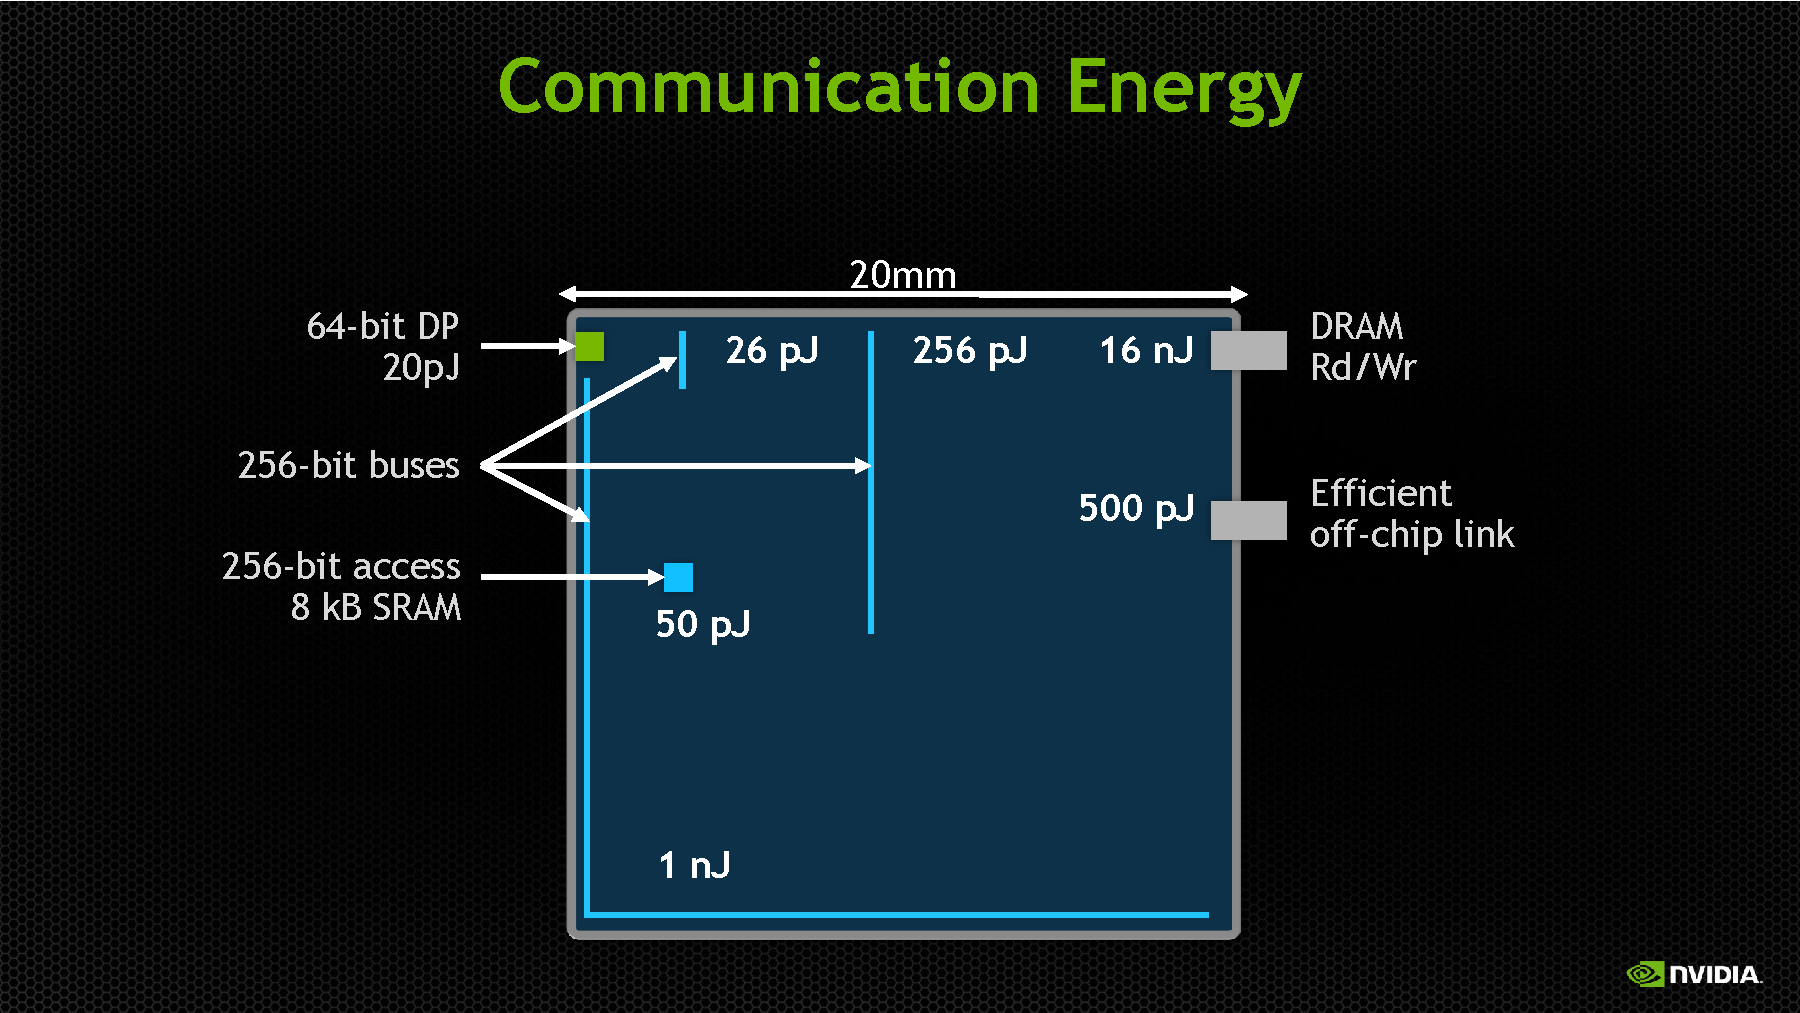
\includegraphics[width=\textwidth,clip,trim=0 0 0 3.5cm]{nvidia.pdf}
    \footnotesize (image : Bill Dally, NVIDIA, `` the path to exascale'')
  \end{center}

  \begin{block}{On a usual CPU}
    \begin{itemize}
    \item Read RAM = 10$\times$ FP64 multiplication
    \end{itemize}
  \end{block}
\end{frame}

%%%%%%%%%%%%%%%%%%%%%%%%%%%%%%%%%%%%%%%%%%%%%%%%%%%%%%%%%%

\begin{frame}[fragile,label=pointer_jumping]
  \frametitle{Non-contiguous Accesses}

  $T =$ array of $N$ random integers in $[0; N)$

  \smallskip
  
\begin{minted}[fontsize=\small]{C}
for (int i=0, x=0; i < 1000000000; i++) x = T[x];
\end{minted}
\begin{overlayarea}{\textwidth}{6.5cm}
  \begin{onlyenv}<1>
    \bigskip
    \begin{exampleblock}{In theory}
      Complexity independent of $N$
    \end{exampleblock}

    \medskip

    \begin{alertblock}{In practice}
      We are dealing with memory \textbf{latency}
    \end{alertblock}

\end{onlyenv}
  \begin{onlyenv}<2->
    \begin{center}
      \vspace{-0.33cm}
      \begin{tikzpicture}
        \node[anchor=south west] at (0, 0) {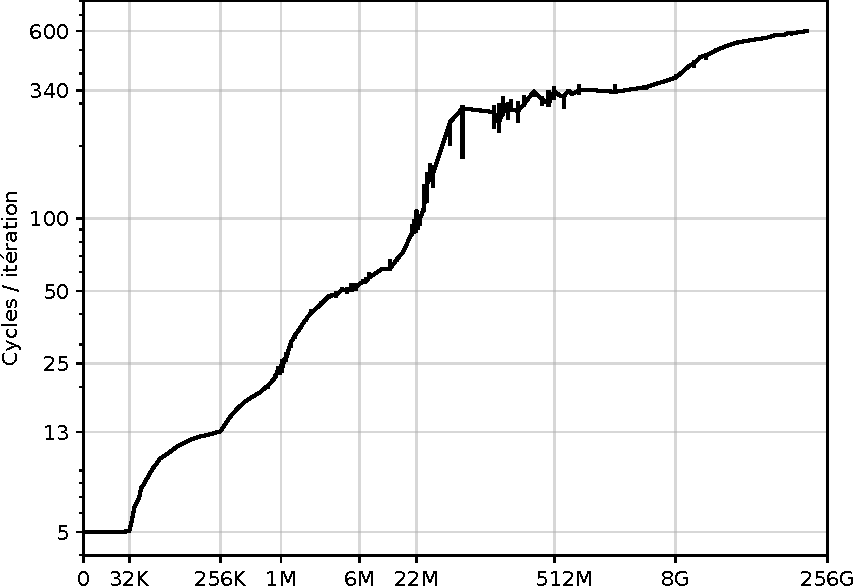
\includegraphics[height=6.5cm]{cache_curve_gr20.pdf}};
        \draw[Green] (1.2, 6.33) node[right] {Contiguous access: 13GB/s};
        \draw<3->[thick,red,->] (1.4, 4) node[right] {3GB/s} -- +(0, -3.15);
        \draw<4->[thick,red,->] (6.32, 1.33) node[left] {48MB/s} -- +(0, 4.1);
        \draw<5->[thick,red,->] (9, 1.33) node[left] {27MB/s} -- +(0, 4.9);
      \end{tikzpicture}
    \end{center}
\end{onlyenv}
\end{overlayarea}
\end{frame}

%%%%%%%%%%%%%%%%%%%%%%%%%%%%%%%%%%%%%%%%%%%%%%%%%%%%%%%%%%

\begin{frame}<1-2>[label=plan]
  \frametitle{Roadmap}

  \begin{enumerate}
  \item<alert@2> The hardware

    \bigskip
    
  \item Memory hierarchy (caches)

    \bigskip

  \item Improving data locality

    \bigskip

  \item (bonus) Paging-related issues
  \end{enumerate}
  
\end{frame}



\section{Hardware}


\begin{frame}
  \frametitle{A \emph{DIMM} (a `` memory stick'')}

  \vfill
  \begin{tikzpicture}[every node/.style={font=\small}, invisible/.style={opacity=0}]
    \path[red,dotted,use as bounding box] (0.2, -4.75) rectangle +(\textwidth, 7.5);
    \node[anchor=south west] at (0, 0) {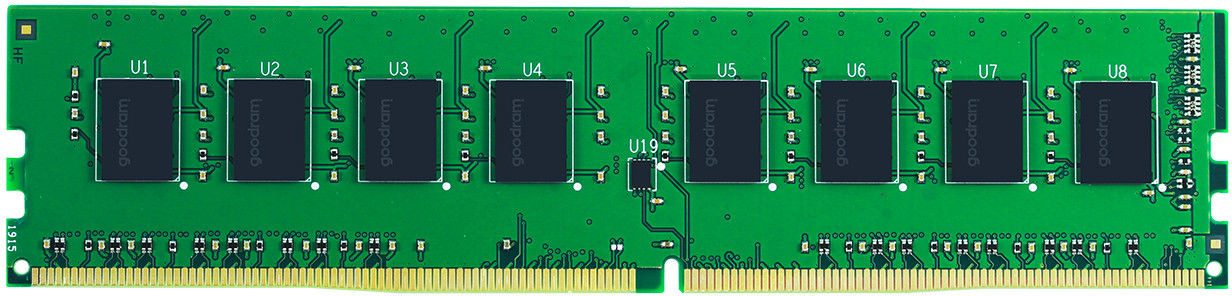
\includegraphics[width=\textwidth]{DIMM.jpg}};

    \foreach \i in {1.025, 2.15, 3.3, 4.45, 6.1725, 7.3, 8.45, 9.575} {
      \draw<2->[yellow, very thick] (\i, 1.2) rectangle +(0.75, 0.9);
      \draw<5->[cyan, very thick] (\i + 0.2, 1.2) -- +(0, -0.66);
      \draw<4>[cyan, very thick, ->] (\i + 0.2, 1.2) -- +(0, -1.25) node[below,font=\footnotesize] {8 bits};
      \draw<3,5->[orange, very thick,<-] (\i + 0.6, 1.2) -- +(0, -0.33);
    }

    % barres horizontales
    \draw<3,5->[orange, very thick] (1.025 + 0.6, 1.2 -0.33) -- (9.575 + 0.6, 1.2 - 0.33) ;
    \draw<5->[cyan, very thick]     (1.025 + 0.2, 1.2 -0.66) -- (9.575 + 0.2, 1.2 - 0.66) ;

    \node[orange, anchor=north]             at (7.33625, -0.5) (ad) {\only<3,5->{address}};
    \node[cyan, anchor=north, align=center] at (3.875,   -0.5) (do) {\only<5->{data \\ (64 bits/cycle)}};

    \draw (5.605625, -2.5) node (ca) {\only<6->{channel}};

    % flèche des barres horizontales vers "données", "adresse"
    \draw<3,5->[orange, very thick] (6.73625+0.6,  1.2 - 0.33) edge (ad);
    \draw<5->[cyan, very thick] (3.3+0.2+0.375, 1.2 - 0.66) edge[->] (do);

    \draw<6->[orange, very thick, <-] (ad) edge (ca);
    \draw<6->[cyan, very thick, <->]  (do) edge (ca);
    
    \draw (5.6, -4.25) node (ctrl) {\only<7->{memory controller}};
    \draw<7->[very thick,->] (ctrl) edge[transform canvas={xshift=-2mm}] (ca);
    \draw<7->[very thick,->] (ca)   edge[transform canvas={xshift=+2mm}] (ctrl);
  \end{tikzpicture}
  \vfill
\end{frame}

%%%%%%%%%%%%%%%%%%%%%%%%%%%%%%%%%%%%%%%%%%%%%%%%%%%%%%%%%%%%%%%%%%%%%%%%

\begin{frame}
  \frametitle{A \emph{DIMM} (a `` memory stick'')}

  \begin{tikzpicture}[every node/.style={font=\small}, invisible/.style={opacity=0}]
    \path[red,dotted,use as bounding box] (0.2, -0.5) rectangle +(\textwidth, 3);
    \node[anchor=south west] at (0, 0) {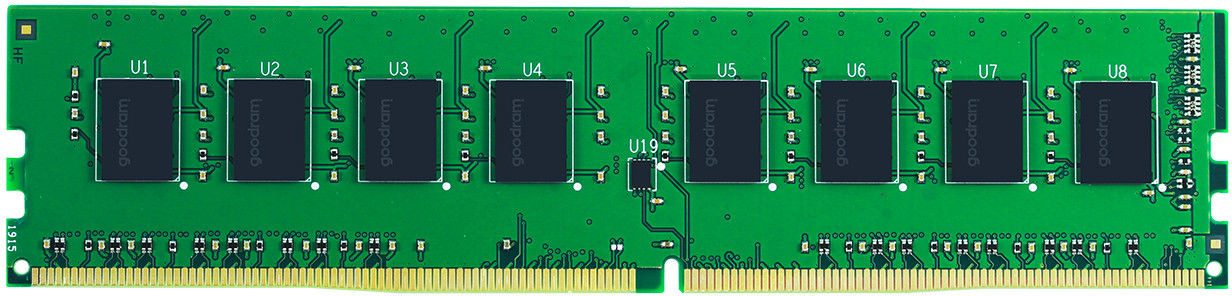
\includegraphics[width=\textwidth]{DIMM.jpg}};
  \end{tikzpicture}

  \vfill
  
  \centering\small
  \begin{tabular}{|c|c|c|c|c|}
  \hline
  Generation     & Year & Mhz       & Prefetch  & GB/s \\
  \hline\hline                                                    
  DDR\phantom{1} & 2000  & 100--200  & 16        &  1.6--3.2 \\
  \hline                                                          
  DDR2           & 2003  & 100--266  & 32        &  3.2--8.5 \\
  \hline                                                          
  DDR3           & 2007  & 100--266  & 64        &  6.4--17 \\
  \hline                                                          
  DDR4           & 2014  & 200--400  & 64        &  12.8--25.6 \\
    \hline
\end{tabular}
\vfill
\end{frame}

%%%%%%%%%%%%%%%%%%%%%%%%%%%%%%%%%%%%%%%%%%%%%%%%%%%%%%%%%%%%%%%%%%%%%%%%

\begin{frame}
  \frametitle{Memory Channels}
  \framesubtitle{More parallelism, more bandwidth}

  \tikzset{
    -|/.style={to path={-| (\tikztotarget)}},
    |-/.style={to path={|- (\tikztotarget)}},
  }
  
  \begin{tikzpicture}[every node/.style={font=\small}]
    \node<1>[anchor=west] at (-1.5, 4) {$\leq$ 2000};
    \node<2>[anchor=west] at (-1.5, 4) {$\geq$ 2000, almost all ``consummer'' CPUs (Core i3, i5, ...)};
    \node<3>[anchor=west] at (-1.5, 4) {2008, Core i7 920 `` Bloomfield''};
    \node<4>[anchor=west] at (-1.5, 4) {2010, AMD Opteron 6100, AMD Ryzen, Core i7/i9 ``X series''};
    \node<5>[anchor=west] at (-1.5, 4) {2017, Xeon Scalable (`` Skylake'')};
    \node<6>[anchor=west] at (-1.5, 4) {2019, AMD Epyc, IBM Power9};
    
    \path[red,dotted,use as bounding box] (-1.6, -3) rectangle +(11, 4);
    \node<1,3,5,6> at (4, 3) (DIMM0) {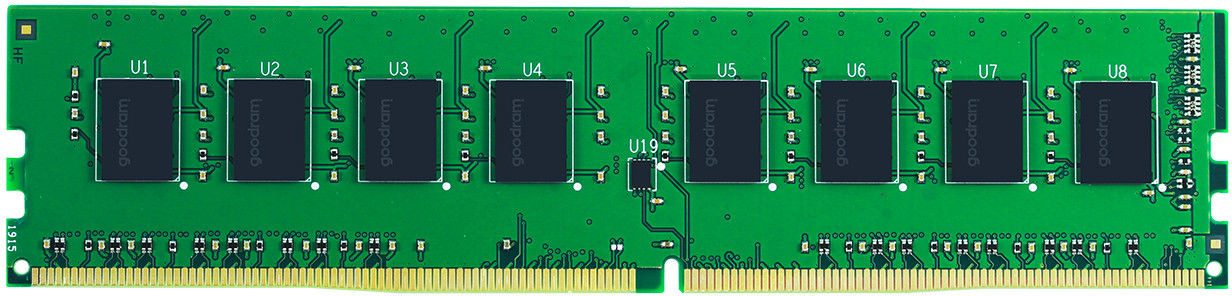
\includegraphics[width=0.25\textwidth]{DIMM.jpg}};

    \node<2,4> at (1, 3) (DIMM1) {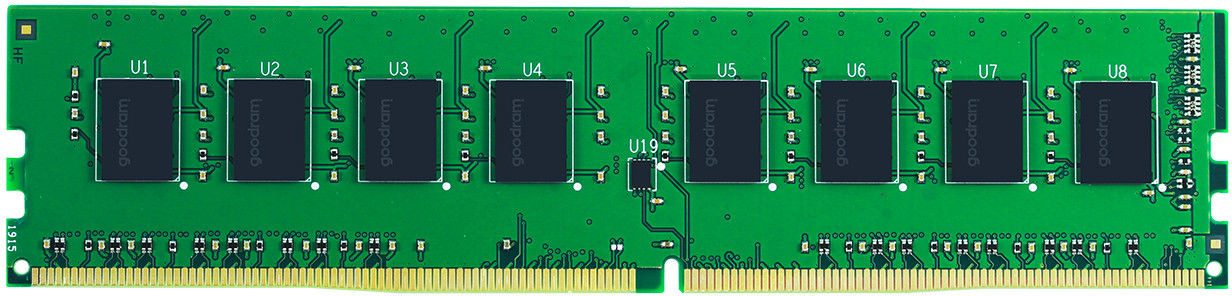
\includegraphics[width=0.25\textwidth]{DIMM.jpg}};
    \node<2,4> at (7, 3) (DIMM2) {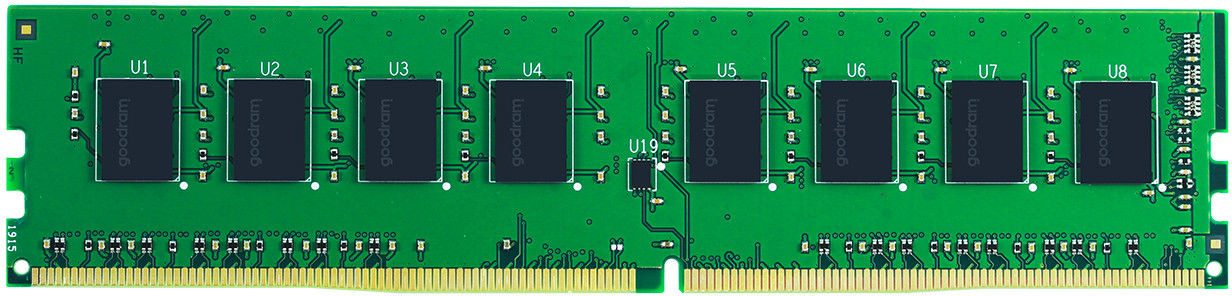
\includegraphics[width=0.25\textwidth]{DIMM.jpg}};

    \node<3,5,6> at (0, 3) (DIMM3) {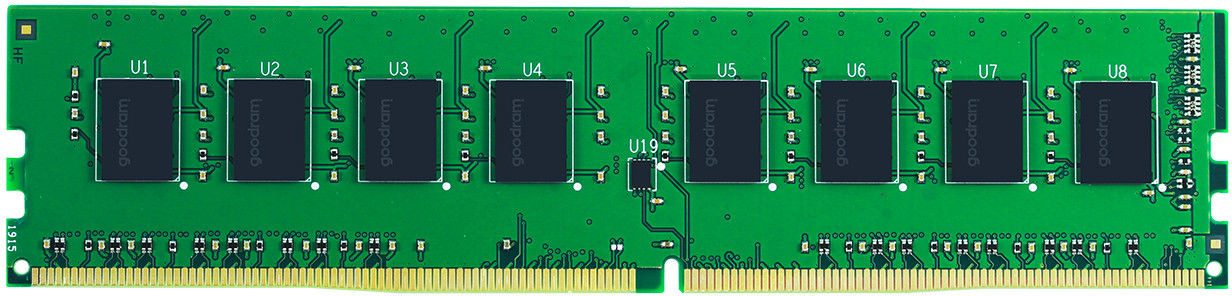
\includegraphics[width=0.25\textwidth]{DIMM.jpg}};
    \node<3,5,6> at (8, 3) (DIMM5) {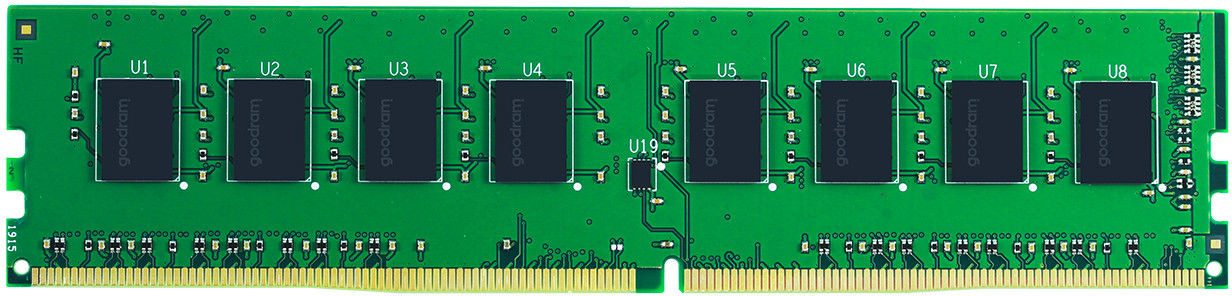
\includegraphics[width=0.25\textwidth]{DIMM.jpg}};

    \node<4> at (1, -3) (DIMM6) {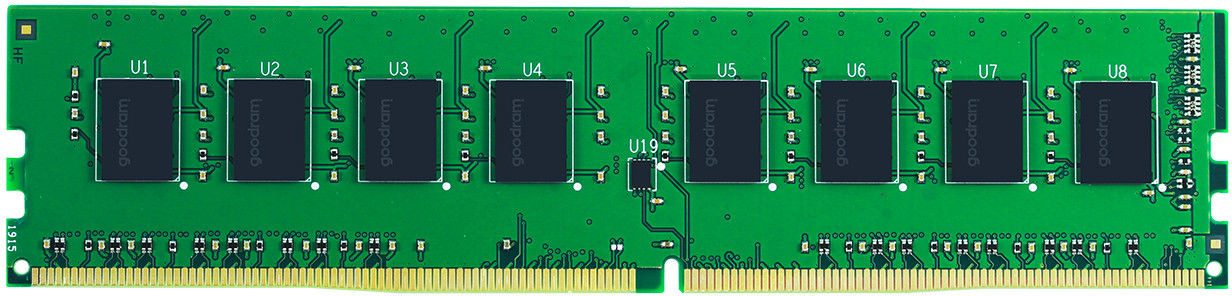
\includegraphics[width=0.25\textwidth]{DIMM.jpg}};
    \node<4> at (7, -3) (DIMM7) {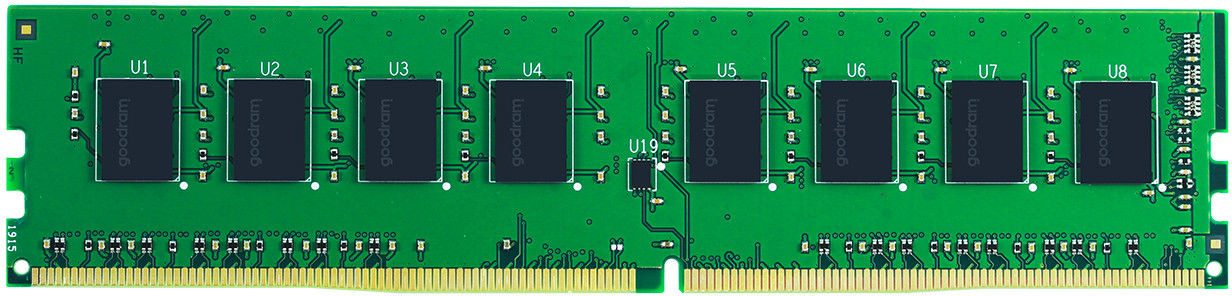
\includegraphics[width=0.25\textwidth]{DIMM.jpg}};

    \node<5,6> at (0, -3) (DIMM8) {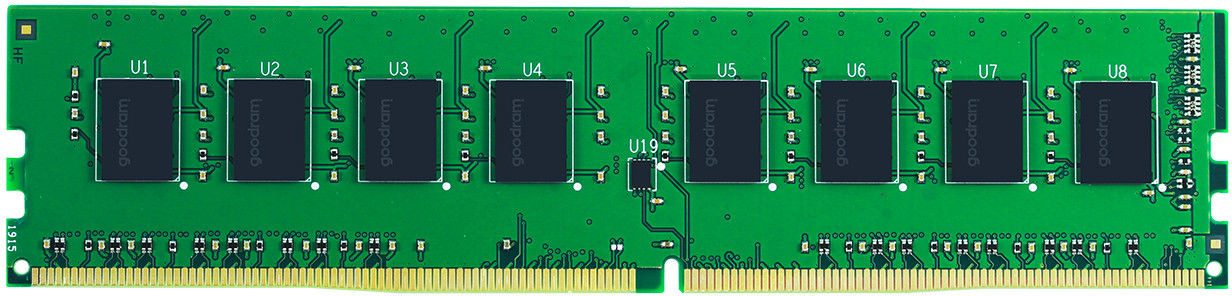
\includegraphics[width=0.25\textwidth]{DIMM.jpg}};
    \node<5,6> at (4, -3) (DIMM9) {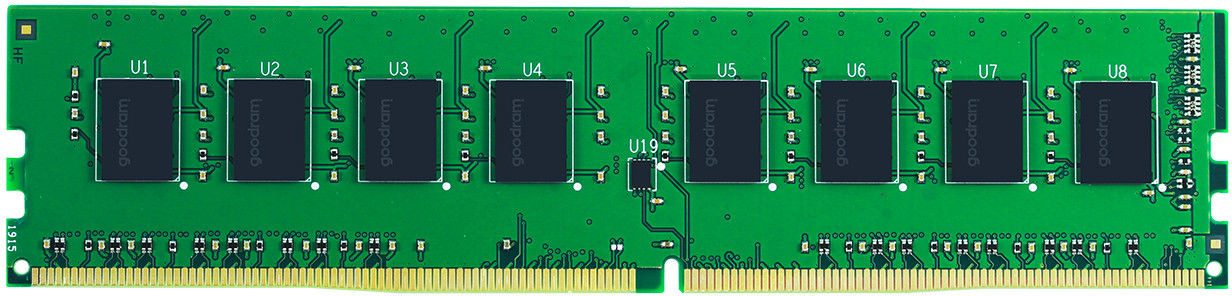
\includegraphics[width=0.25\textwidth]{DIMM.jpg}};
    \node<5,6> at (8, -3) (DIMMa) {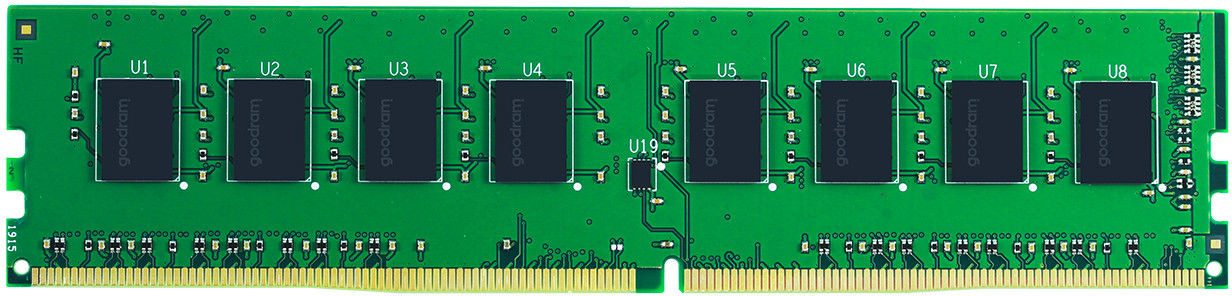
\includegraphics[width=0.25\textwidth]{DIMM.jpg}};


    \node<6> at (0, 0) (DIMMb) {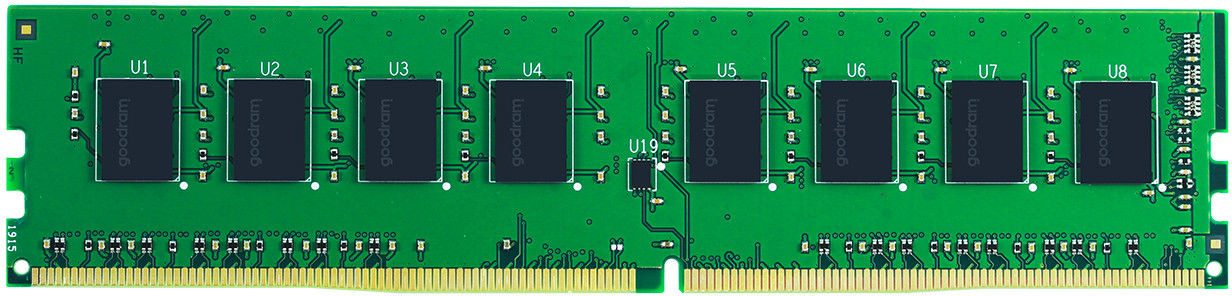
\includegraphics[width=0.25\textwidth]{DIMM.jpg}};
    \node<6> at (8, 0) (DIMMc) {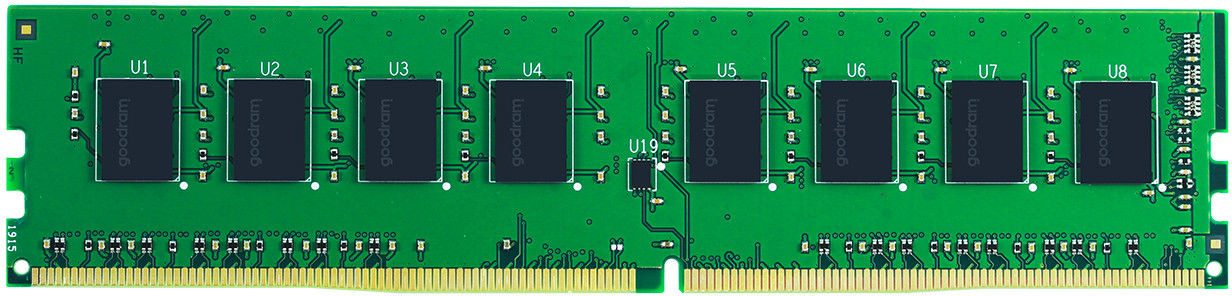
\includegraphics[width=0.25\textwidth]{DIMM.jpg}};

    
    \node[draw,thick] at (4, 0) (cntrl) {Memory controller};
    
    \draw<1>[thick] (cntrl) -- node[right] {Channel 0} (DIMM0);

    \draw<2>[thick] (cntrl)  -| node[near end, left] {Channel 0} (DIMM1);
    \draw<2>[thick] (cntrl)  -| node[near end, right] {Channel 1} (DIMM2);

    \draw<3>[thick] (cntrl)  -| node[near end, left] {Channel 0} (DIMM3);
    \draw<3>[thick] (cntrl)  -- node[right] {Channel 1} (DIMM0);
    \draw<3>[thick] (cntrl)  -| node[near end, right] {Channel 2} (DIMM5);

    \draw<4>[thick,transform canvas={yshift=+1mm}] (cntrl)  -| node[near end, left] {Channel 0} (DIMM1);
    \draw<4>[thick,transform canvas={yshift=+1mm}] (cntrl)  -| node[near end, left] {Channel 1} (DIMM2);
    \draw<4>[thick,transform canvas={yshift=-1mm}] (cntrl)  -| node[near end, left] {Channel 2} (DIMM6);
    \draw<4>[thick,transform canvas={yshift=-1mm}] (cntrl)  -| node[near end, right] {Channel 3} (DIMM7);

    \draw<5>[thick,transform canvas={yshift=+1mm}] (cntrl)  -| node[near end, left] {Channel 0} (DIMM3);
    \draw<5>[thick] (cntrl)  -- node[right] {Channel 1} (DIMM0);
    \draw<5>[thick,transform canvas={yshift=+1mm}] (cntrl)  -| node[near end, right] {Channel 2} (DIMM5);
    \draw<5>[thick,transform canvas={yshift=-1mm}] (cntrl)  -| node[near end, left] {Channel 3} (DIMM8);
    \draw<5>[thick] (cntrl)  -- node[right] {Channel 4} (DIMM9);
    \draw<5>[thick,transform canvas={yshift=-1mm}] (cntrl)  -| node[near end, right] {Channel 5} (DIMMa);
    
    \draw<6>[thick,transform canvas={yshift=+1mm}] (cntrl)  -- node[near end, left] {Channel 0} (DIMM3);
    \draw<6>[thick] (cntrl)  -- node[right, near end] {Channel 1} (DIMM0);
    \draw<6>[thick] (cntrl)  --  (DIMMb);
    \draw<6>[thick,transform canvas={yshift=+1mm}] (cntrl)  -- node[near end, right] {Channel 2} (DIMM5);
    \draw<6>[thick,transform canvas={yshift=-1mm}] (cntrl)  -- node[near end, left] {Channel 5} (DIMM8);
    \draw<6>[thick] (cntrl)  -- node[right,near end] {Channel 6} (DIMM9);
    \draw<6>[thick] (cntrl)  --  (DIMMc);
    \draw<6>[thick,transform canvas={yshift=-1mm}] (cntrl)  -- node[near end, right] {Channel 7} (DIMMa);

 \end{tikzpicture}
\end{frame}

%%%%%%%%%%%%%%%%%%%%%%%%%%%%%%%%%%%%%%%%%%%%%%%%%%%%%%%%%%%%%%%%%%%%%%%%


\begin{frame}
  \frametitle{Closer, Faster}

  \begin{tikzpicture}[every node/.style={font=\small}]
    \node<1> at (4, 4) {$\leq$ 2008 : controller on the motherboard (`` chipset, north bridge'')};
   \node<3>[anchor=west] at (-1.5, 4) {$\geq$ 2008, controller on the CPU};
    
    \path[red,dotted,use as bounding box] (-1.4, -2.5) rectangle +(11.5, 7);
    \node<1> at (8, 0) (DIMM0) {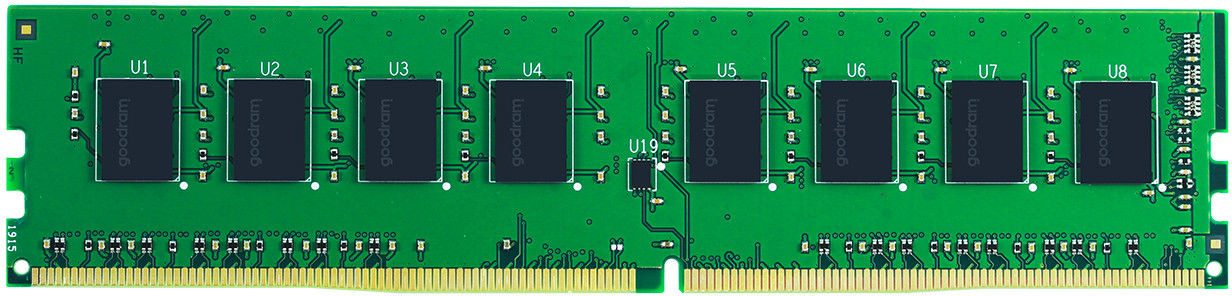
\includegraphics[width=0.25\textwidth]{DIMM.jpg}};
    \node<1> at (-1, 0) (cpu) {
\includegraphics[width=2cm]{cpu_clipart.png}};
    \node<1>[draw,thick] at (3.25, 0) (cntrl) {memory controller};
    \draw<1> (cpu) -- (cntrl);
    \draw<1> (cntrl) -- (DIMM0);

    \node<2>[inner sep=0] at (4, 0) {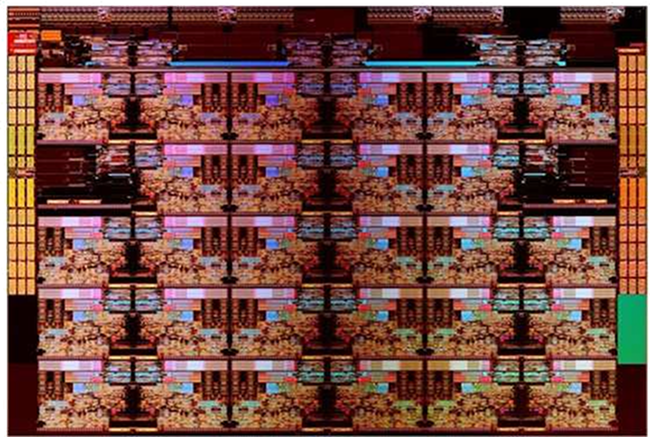
\includegraphics[width=6cm]{650px-skylake-sp_xcc_die_shot.png}};
    \node<3>[inner sep=0] (xeon) at (4, 0)  {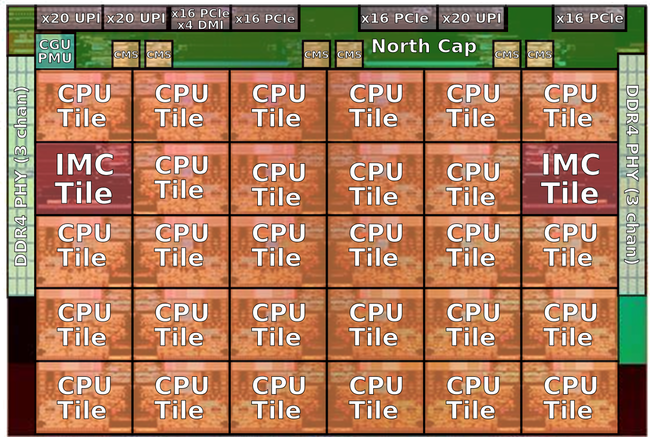
\includegraphics[width=6cm]{650px-skylake-sp_xcc_die_shot_annotated.png}};

    \node<3> at (9, 2) (DIMM0) {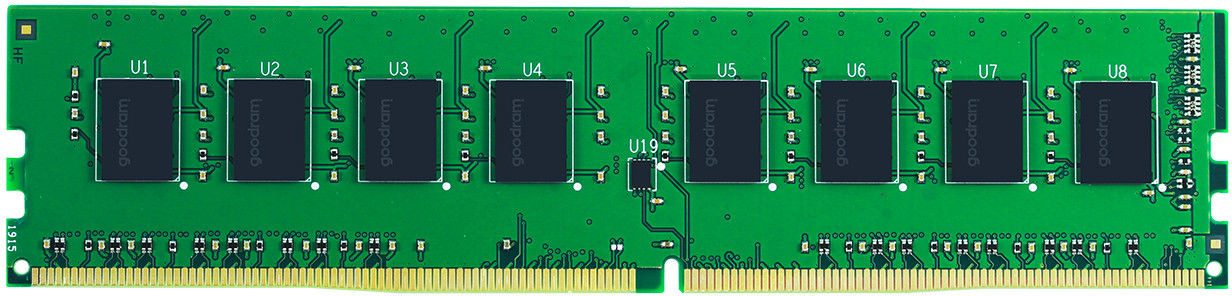
\includegraphics[width=2cm]{DIMM.jpg}};
    \node<3> at (9, 0) (DIMM1) {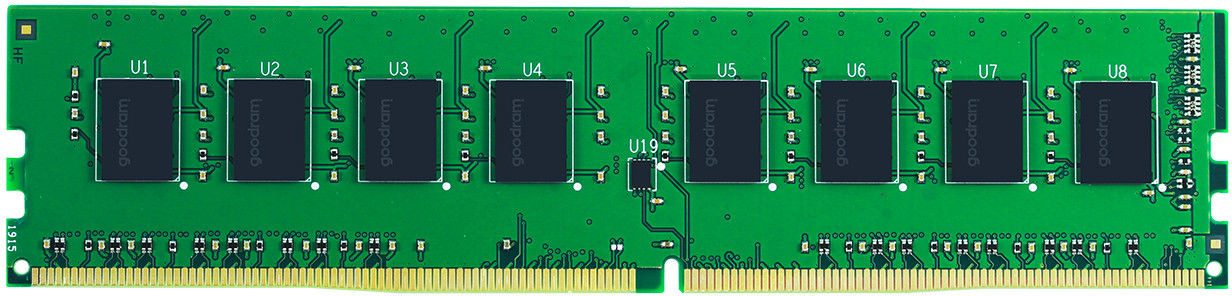
\includegraphics[width=2cm]{DIMM.jpg}};
    \node<3> at (9, -2) (DIMM2) {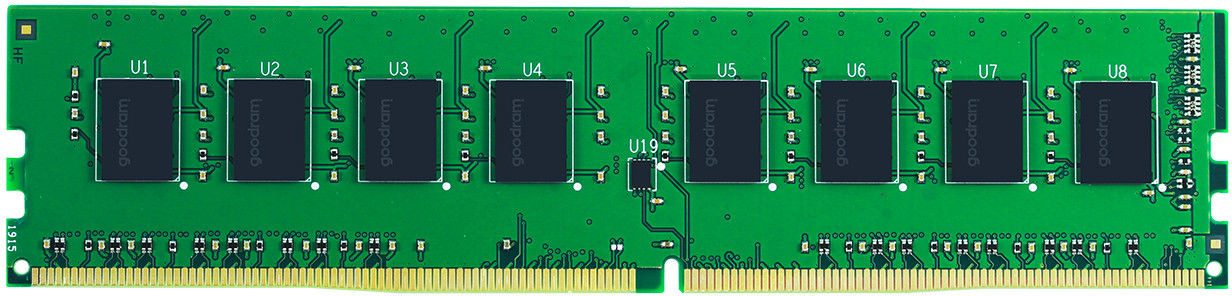
\includegraphics[width=2cm]{DIMM.jpg}};

    \node<3> at (-1, 2) (DIMM3) {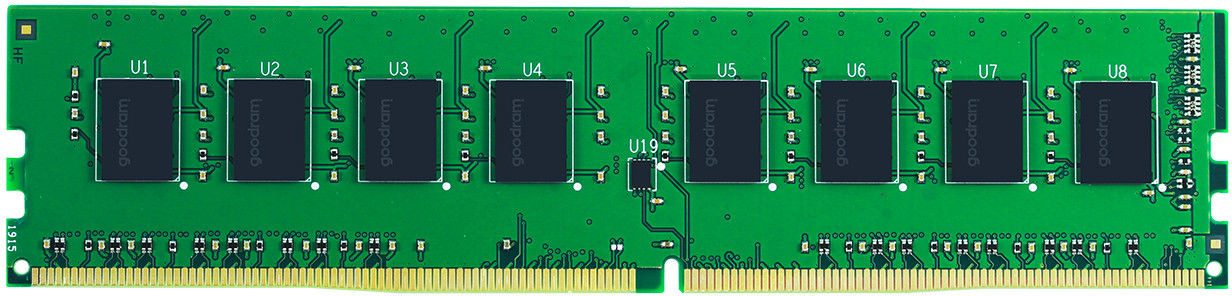
\includegraphics[width=2cm]{DIMM.jpg}};
    \node<3> at (-1, 0) (DIMM4) {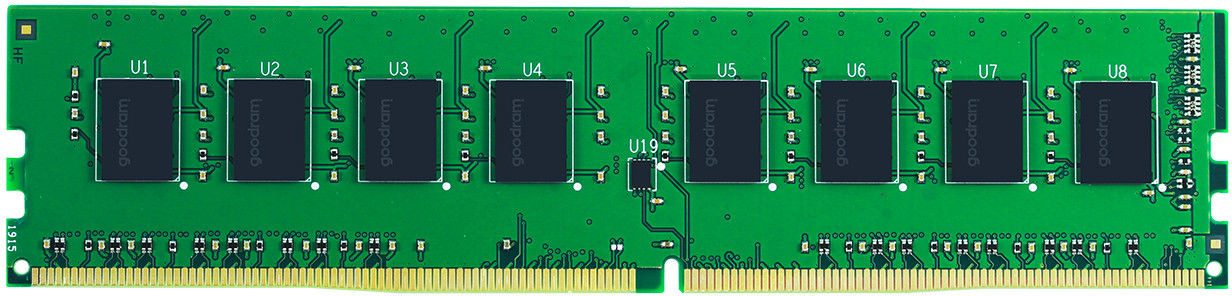
\includegraphics[width=2cm]{DIMM.jpg}};
    \node<3> at (-1, -2) (DIMM5) {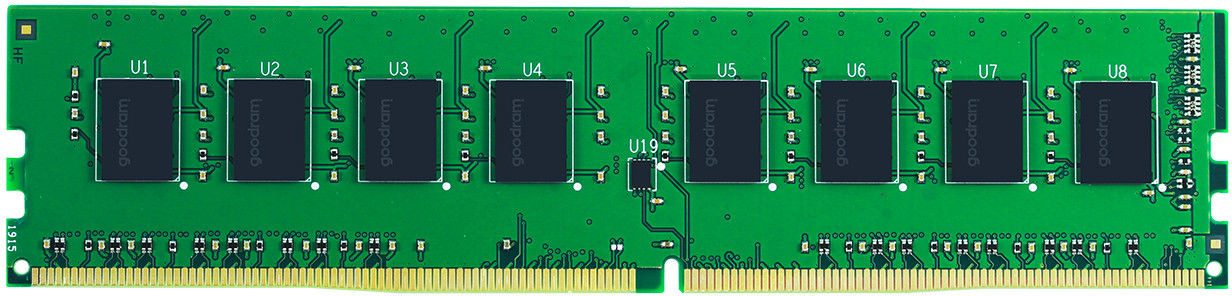
\includegraphics[width=2cm]{DIMM.jpg}};    

    \draw<3> (xeon.west) \foreach \i in {3, 4, 5} {edge (DIMM\i)};
    \draw<3> (xeon.east) \foreach \i in {0, 1, 2} {edge (DIMM\i)};
  \end{tikzpicture}    
\end{frame}


%%%%%%%%%%%%%%%%%%%%%%%%%%%%%%%

\begin{frame}
  \frametitle{In greater detail}

  \vfill
    \begin{tikzpicture}

      \node[anchor=south west] at (0, 0) {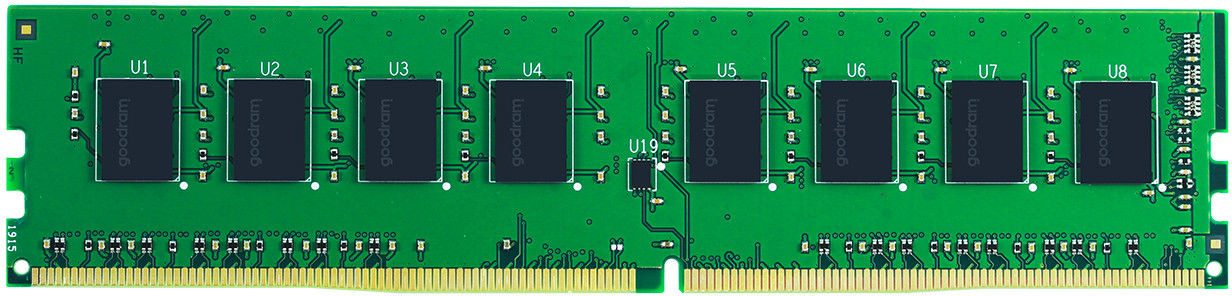
\includegraphics[width=\textwidth]{DIMM.jpg}};

      \foreach \i in {1.025, 2.15, 3.3, 4.45, 6.1725, 7.3, 8.45, 9.575} {
        \draw<2->[yellow, very thick] (\i, 1.2) rectangle +(0.75, 0.9);
      }
    \end{tikzpicture}
    \vfill
    
\end{frame}



%%%%%%%%%%%%%%%%%%%%%%%%%%%%%%%%%%%%%%%%%%

\begin{frame}<1>[label=banks]
  \frametitle{Rows, Columns and Banks}

  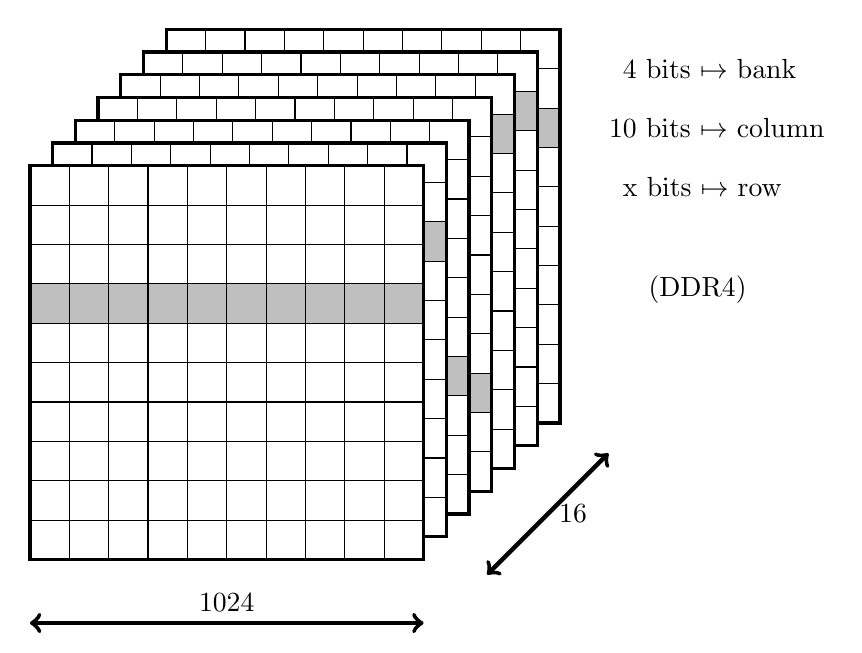
\begin{tikzpicture}[scale=0.5]
    % \draw[fill=lightgray] (0, 8, 0) rectangle +(10, 1);
    % \draw[fill=lightgray] (0, 3, 1.5) rectangle +(10, 1);
    % \draw[fill=lightgray] (0, 5, 3) rectangle +(10, 1);
    % \draw[fill=lightgray] (0, 8, 4.5) rectangle +(10, 1);
    % \draw[fill=lightgray] (0, 1, 6) rectangle +(10, 1);
    % \draw[fill=lightgray] (0, 8, 7.5) rectangle +(10, 1);
    % \draw[fill=lightgray] (0, 0, 9) rectangle +(10, 1);
    
    \pgfmathsetseed{42}
    \foreach \z in {0, 1.5, 3, 4.5, 6, 7.5, 9} {

      \pgfmathsetmacro{\i}{random(0,10)}
      \draw[fill=white] (0, 0, \z) rectangle +(10, 10, 0);
      \draw<2>[fill=lightgray] (0, \i, \z) rectangle +(10, 1);
      \draw[very thick] (0, 0, \z) rectangle +(10, 10, 0);
      
      \foreach \i in {1,2,3,4,5,6,7,8,9} {
        \draw (\i, 0, \z) -- +(0, 10);
        \draw (0, \i, \z) -- +(10, 0);
      }
    }
    
    \draw[ultra thick,<->] (-0.385, -2, 8) -- node[above] {1024} +(10, 0);
    \draw[ultra thick,<->] (12, 0, 10) --node[right] {16} +(0, 0, -8);

    \node[anchor=west] at (11, 9) {\phantom{1}4 bits $\mapsto$ bank};
    \node[anchor=west] at (11, 7.5)   {10 bits $\mapsto$ column};
    \node[anchor=west] at (11, 6) {\phantom{1}x bits $\mapsto$ row};

    \node[anchor=west] at (12, 3.4) {(DDR4)};
  \end{tikzpicture}
\end{frame}

%%%%%%%%%%%%%%%%%%%%%%%%%%%%%%%%%%%%%%%%%%

\begin{frame}[label=rows]
  \frametitle{Rows, Columns, ...}

  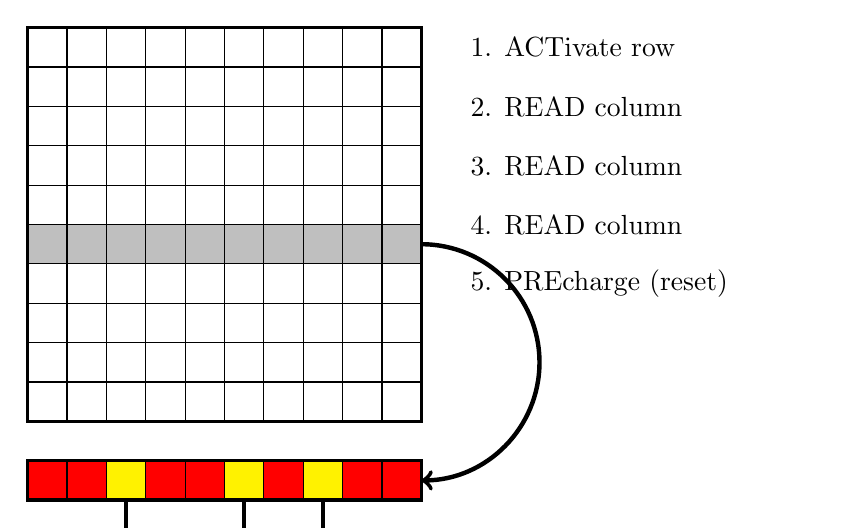
\begin{tikzpicture}[scale=0.5]
    \path[red,dotted,use as bounding box] (0, -2) rectangle +(20, 12);

    \draw<2>[fill=yellow] (2, 4) rectangle +(1, 1);
    \draw<2>[fill=yellow] (5, 4) rectangle +(1, 1);
    \draw<2>[fill=yellow] (7, 4) rectangle +(1, 1);
    
    \draw<3-6>[fill=lightgray] (0, 4) rectangle +(10, 1);
    \draw[very thick] (0, 0) rectangle +(10, 10);
    \draw[very thick,fill=red] (0, -2) rectangle +(10, 1);
%    \draw<3-6>[fill=yellow] (5, -2) rectangle +(3, 1);
    \draw<3-6>[fill=yellow] (2, -2) rectangle +(1, 1);
    \draw<3-6>[fill=yellow] (5, -2) rectangle +(1, 1);
    \draw<3-6>[fill=yellow] (7, -2) rectangle +(1, 1);

    \draw[very thick] (0, -2) rectangle +(10, 1);
    
    \foreach \i in {1,2,3,4,5,6,7,8,9} {
      \draw (\i, -2) -- +(0, 1);
      \draw (\i, 0) -- +(0, 10);
         \draw (0, \i) -- +(10, 0);
       };


       \draw<3>[ultra thick,->] (10, 4.5) arc(90:-90:3);

       \draw<4>[ultra thick,->] (2.5, -2) -- +(0, -1);
       \draw<5>[ultra thick,->] (5.5, -2) -- +(0, -1);
       \draw<6>[ultra thick,->] (7.5, -2) -- +(0, -1);
       
       \node<3->[anchor=west] at (11, 9.5) {1. ACTivate row};
       \node<4->[anchor=west] at (11, 8) {2. READ column};
       \node<5->[anchor=west] at (11, 6.5) {3. READ column};
       \node<6->[anchor=west] at (11, 5.0) {4. READ column};
       \node<7->[anchor=west] at (11, 3.5) {5. PREcharge (reset)};
  \end{tikzpicture}
\end{frame}

%%%%%%%%%%%%%%%%%%%%%%%%%%%%%%%%%%%%%%%%%

\againframe<2>{banks}

%%%%%%%%%%%%%%%%%%%%%%%%%%%%%%%%%%%%%%%%%%

\begin{frame}
  \frametitle{In 2020: DDR4}

    \begin{tikzpicture}
      \node[anchor=south west] at (0, 0) {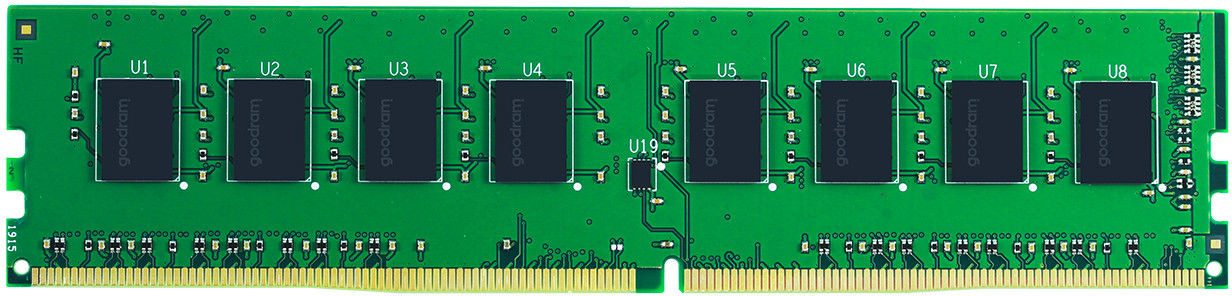
\includegraphics[width=\textwidth]{DIMM.jpg}};
    \end{tikzpicture}
   
  \bigskip
  
  \small
  \begin{tabular}{|c|c|c|c|c|}
  \hline
Standard   & Freq. (Mhz) & GB/s  & CL min. & Latency (ns) \\
  \hline\hline                                                                    
DDR4-1600  & 200         & 12.8 & 10      & 12.5   \\
DDR4-1866  & 233         & 14.9 & 12      & 12.9 \\
DDR4-2133  & 266         & 17.0 & 14      & 13.1 \\
DDR4-2400  & 300         & 19.2 & 15      & 12.5   \\
DDR4-2666  & 333         & 21.3 & 17      & 12.8  \\
DDR4-2933  & 366         & 23.5 & 19      & 13.0  \\
DDR4-3200  & 400         & 25.6 & 20      & 12.5   \\
  \hline                                                                                            
\end{tabular}
\end{frame}


\section{La hiérarchie mémoire}

\againframe<3>{plan}

\begin{frame}[label=caches]
  \frametitle{Memory Hierarchy}

  \begin{tikzpicture}[every node/.style={font=\small}, scale=0.66, node distance=0.5cm]
    \path[use as bounding box] (-8.5, 0) rectangle +(17, 10);
    
    \node at (0, 0) (cpu) {
\includegraphics[width=1cm]{cpu_clipart.png}};
    \node[above=of cpu, shape=rectangle, draw, align=center] (L1) {L1 cache ($\approx$ 32Ko)};
    \node[above=of L1, shape=rectangle, draw, align=center] (L2) {L2 cache (256Ko--1Mo)};
    \node[above=of L2, shape=rectangle, draw, align=center] (L3) {L3 cache ($\leq$ 64Mo)};
    \node[above=of L3, shape=rectangle, draw, align=center] (L4) {L4 cache (rare, IBM z15: 960Mo)};
    \node[above=of L4, shape=rectangle, draw, align=center] (RAM) {RAM};

    \draw (cpu) edge[<->] (L1);
    \draw (L1) edge[<->] (L2);
    \draw (L2) edge[<->] (L3);
    \draw (L3) edge[<->] (L4);
    \draw (L4) edge[<->] (RAM);

    \draw<2>[red, very thick] (L1.south west) edge[->, bend right] node[left] {5 cycles} (cpu);
    \draw<3>[red, very thick] (L2.south west) edge[->, bend right] node[left] {14 cycles} (cpu);
    \draw<4>[red, very thick] (L3.west) edge[->, bend right=60] node[left] {$\approx 50$ cycles} (cpu.west);
    \draw<5>[red, very thick] (RAM.west) edge[->, bend right=90] node[left] {$\approx 200-1000$ cycles} (cpu.west);
    
  \end{tikzpicture}
\end{frame}

%%%%%%%%%%%

\begin{frame}[fragile,label=caches]
  \frametitle{Effect of the Memory Hierarchy}

  $T =$ array of $N$ random integers in $[0; N)$

  \smallskip
  
\begin{minted}[fontsize=\small]{C}
for (int i=0, x=0; i < 1000000000; i++) x = T[x];
\end{minted}

      \begin{center}
      \vspace{-0.33cm}
      \begin{tikzpicture}
        \node[anchor=south west] at (0, 0) {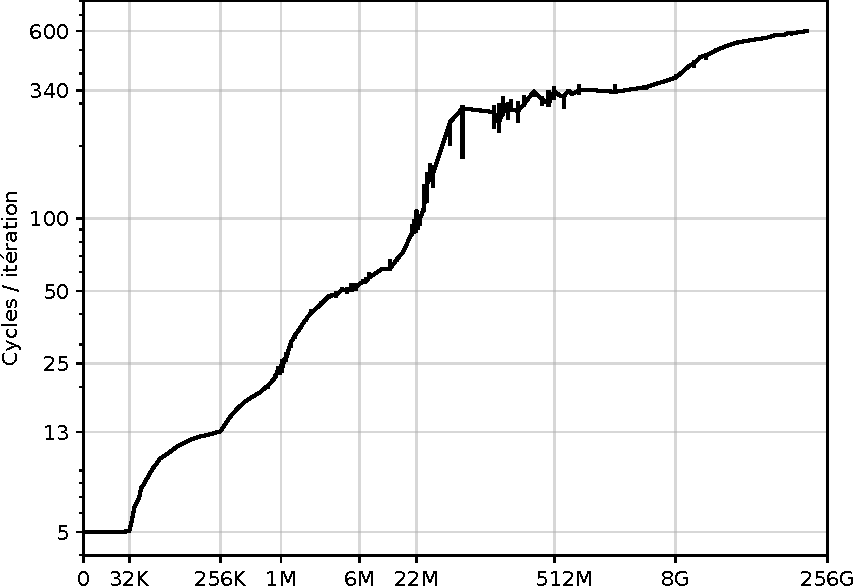
\includegraphics[height=6.5cm]{cache_curve_gr20.pdf}};
        \draw[Green] (1.2, 6.33) node[right] {Contiguous access: 13GB/s};
        \draw<2->[thick,red,->] (1.4, 4) node[right] {3GB/s} -- +(0, -3.15);
        \draw<3->[thick,red,->] (6.32, 1.33) node[left] {48MB/s} -- +(0, 4.1);
        \draw<4->[thick,red,->] (9, 1.33) node[left] {27MB/s} -- +(0, 4.9);
      \end{tikzpicture}
    \end{center}
\end{frame}

%%%%%%%%%%%%%%%%%%%%%%%

\begin{frame}[label=caches]
  \frametitle{Caches: Wide Variety}
  \framesubtitle{Raspberry Pi 3B+ (ARM Cortex A53)}
  \centering
  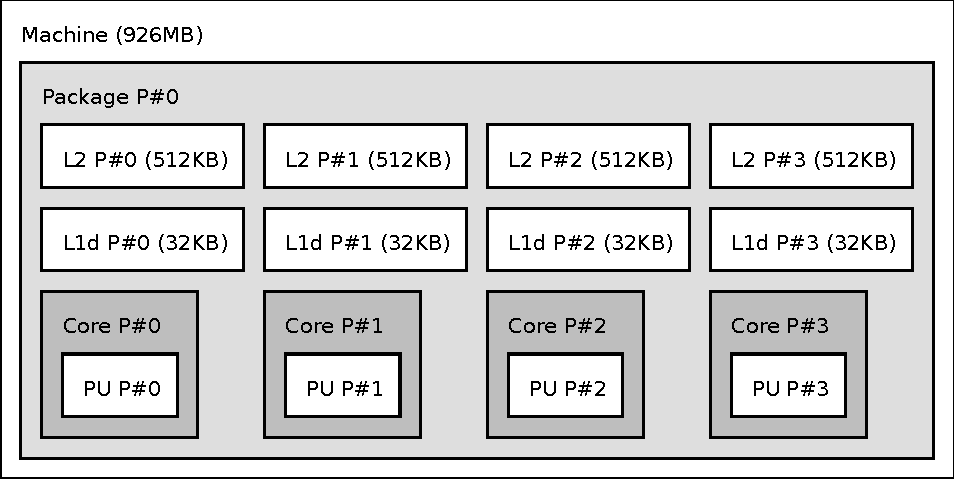
\includegraphics[width=\textwidth]{lstopo_rpi3b.pdf}
\end{frame}

\begin{frame}[label=caches]
  \frametitle{Caches: Wide Variety}
  \framesubtitle{Mon laptop  (Intel Core i7 6600U)}
  \centering
  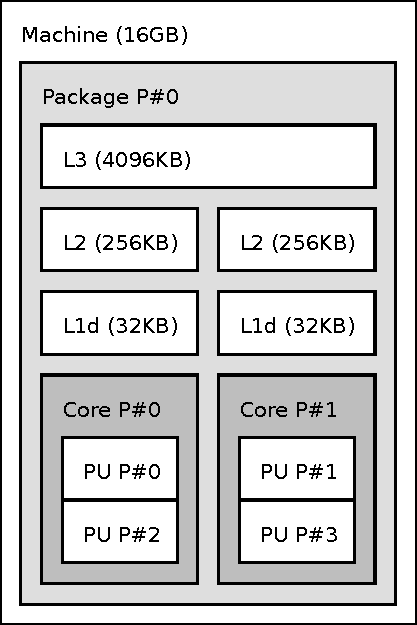
\includegraphics[height=6cm]{lstopo_laptop.pdf}
\end{frame}
  
\begin{frame}[label=caches]
  \frametitle{Caches: Wide Variety}
  \framesubtitle{IBM BlueGene/Q (PowerPC A2)}
  \centering
  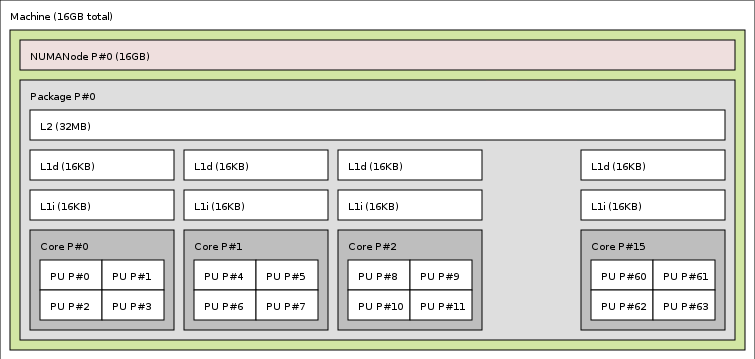
\includegraphics[width=\textwidth]{lstopo_bgq.png}
\end{frame}

\begin{frame}[label=caches]
  \frametitle{Caches: Wide Variety}
  \framesubtitle{Noeud d'un cluster récent (2 $\times$ Intel Xeon Gold 6130)}
  \centering
  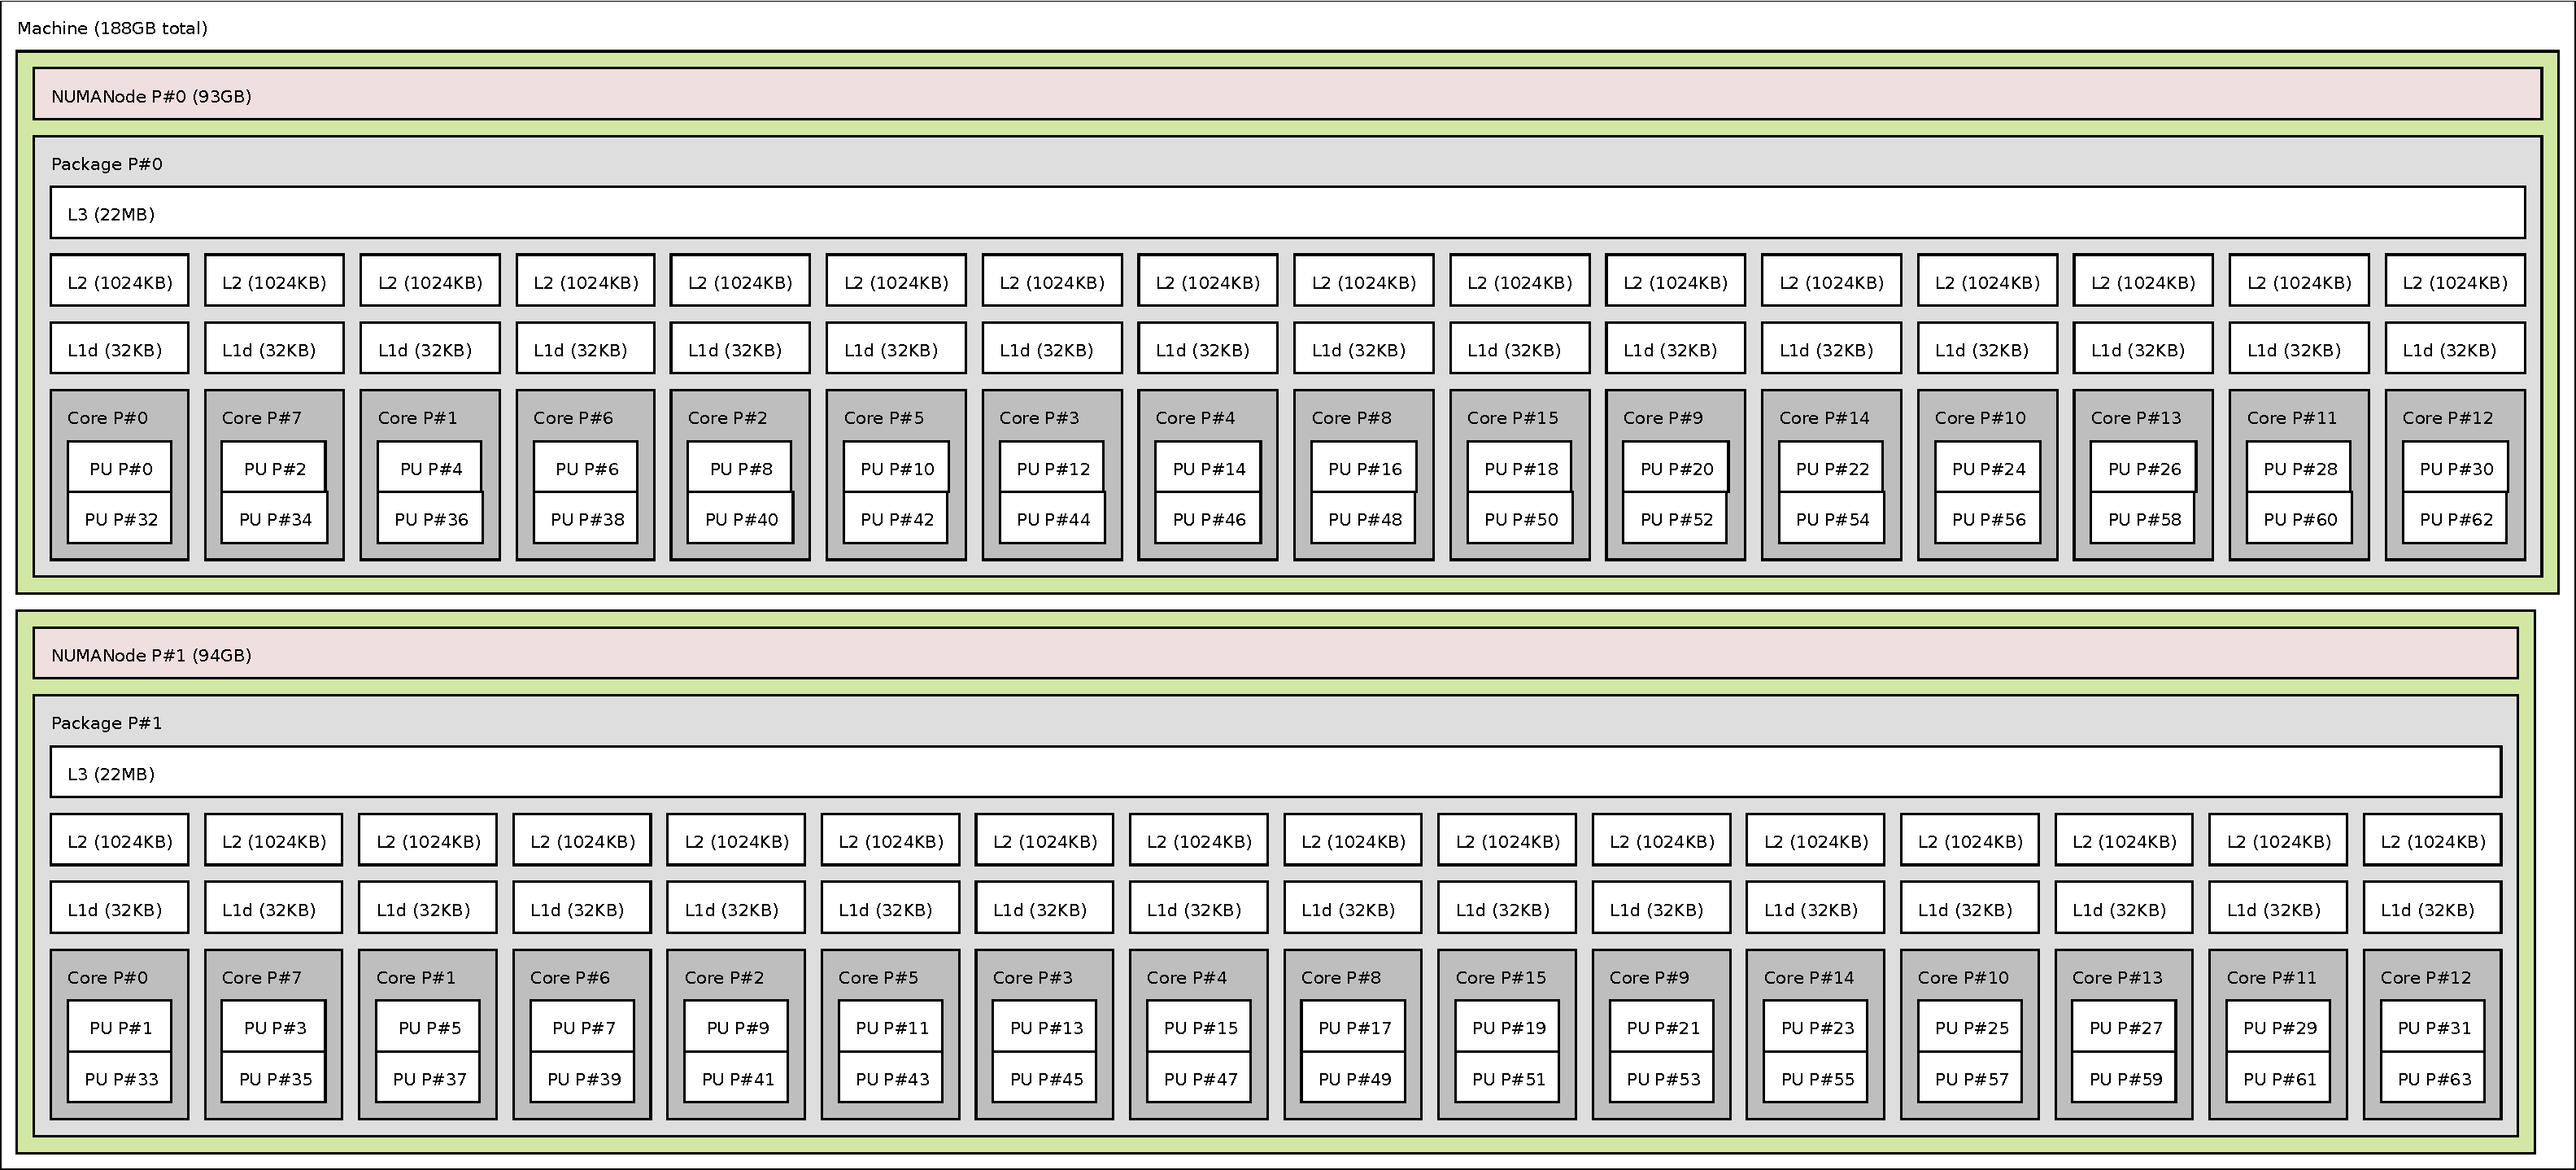
\includegraphics[width=\textwidth]{lstopo_gr20.pdf}
\end{frame}

\begin{frame}[label=caches]
  \frametitle{Caches: Wide Variety}
  \framesubtitle{Noeud d'un autre cluster récent (2 $\times$ AMD EPYC 7301)}
  \centering
  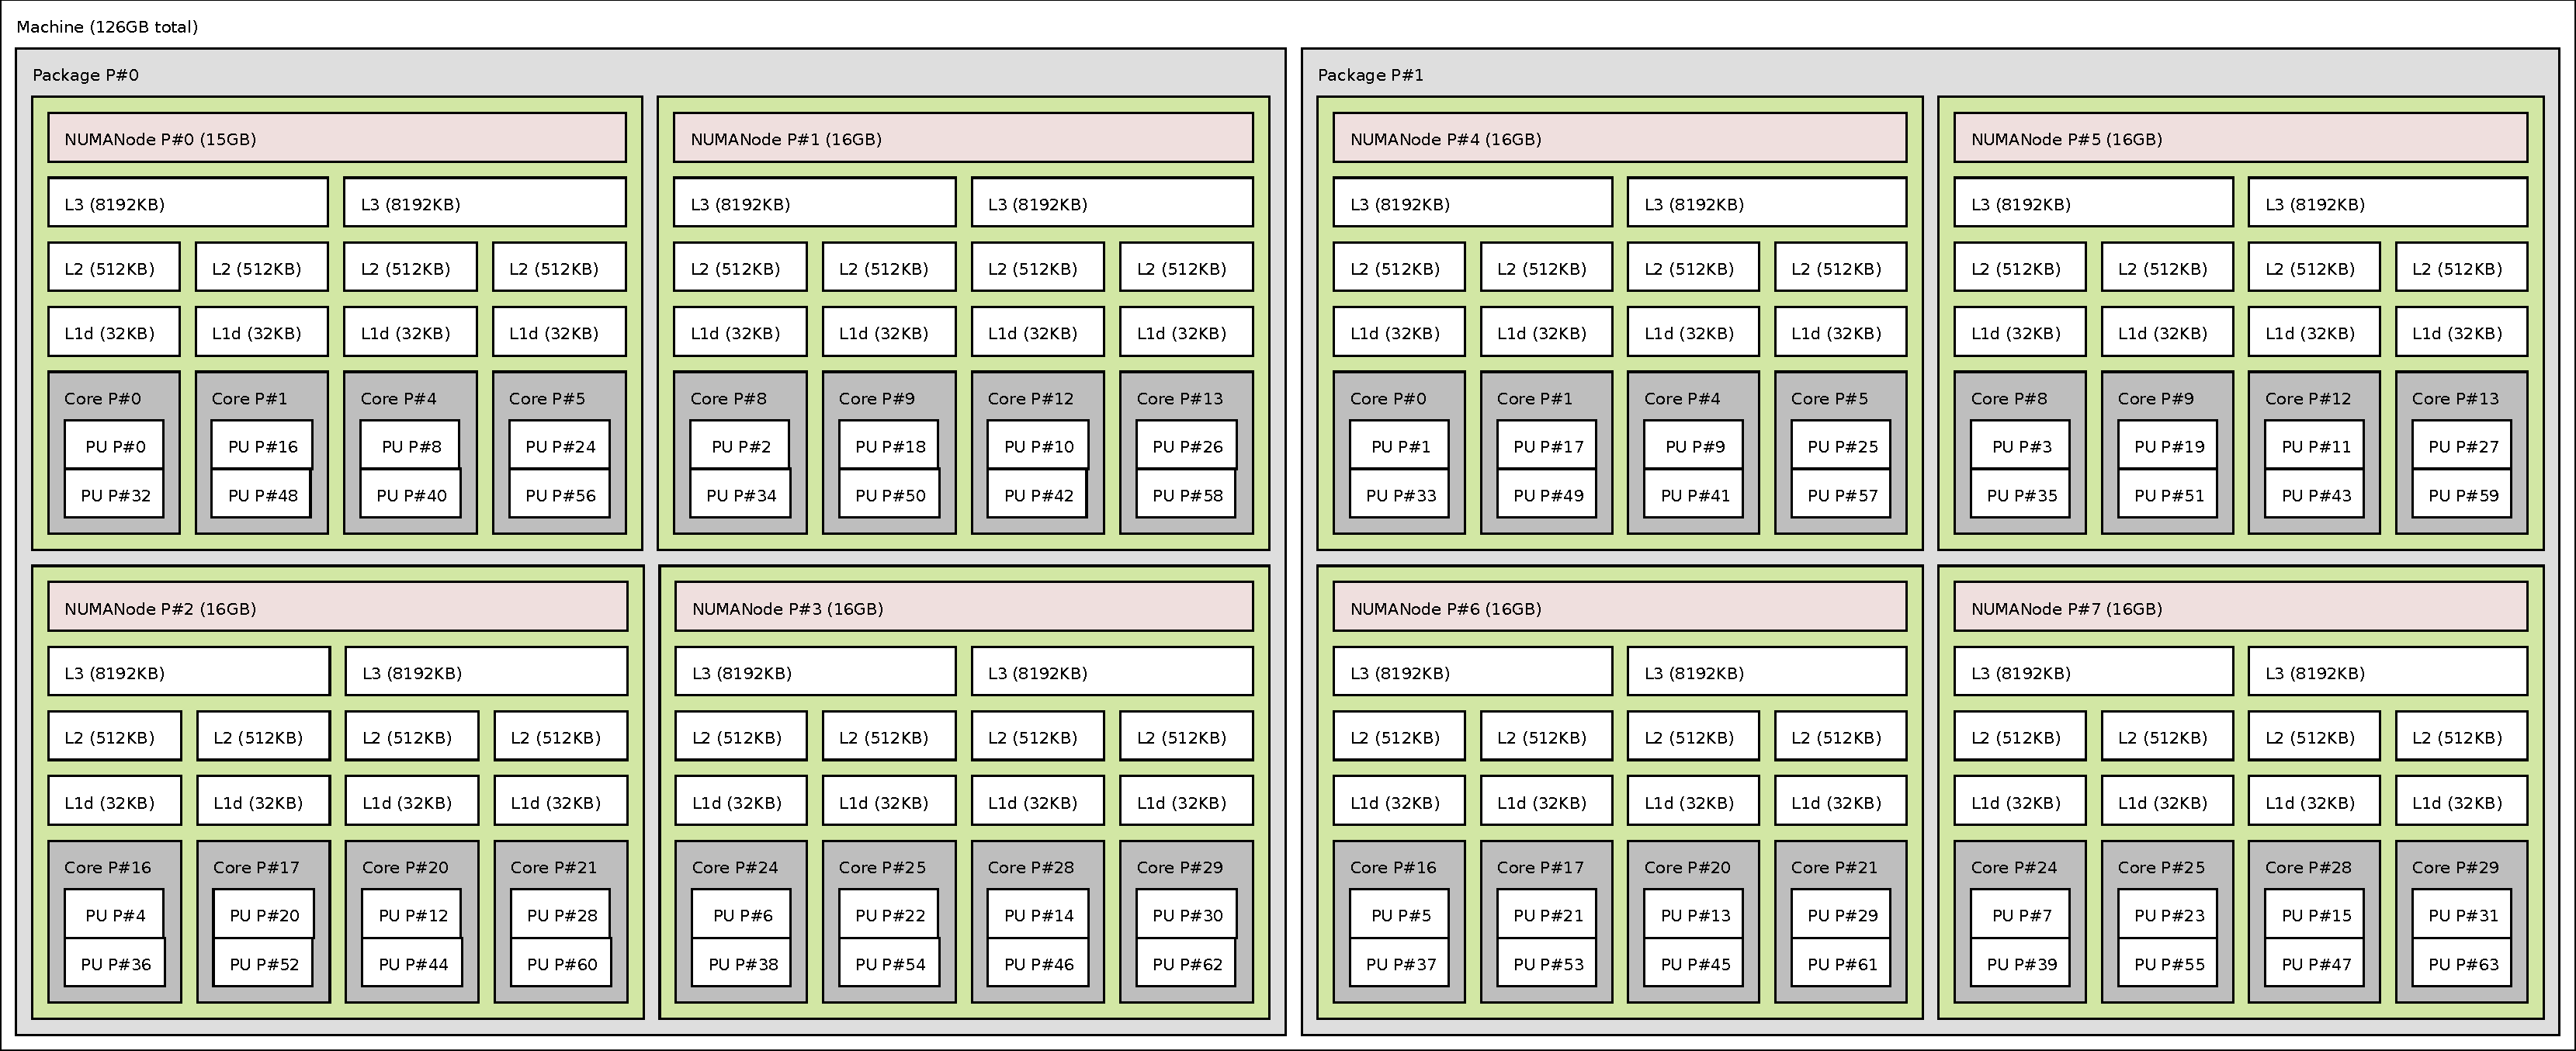
\includegraphics[width=\textwidth]{lstopo_chiclet.pdf}
\end{frame}

\begin{frame}[label=caches]
  \frametitle{Caches: Wide Variety}
  \framesubtitle{Fat Node (4 $\times$ Intel Xeon E7-4850 v3) + 1.5To de RAM}
  \centering
  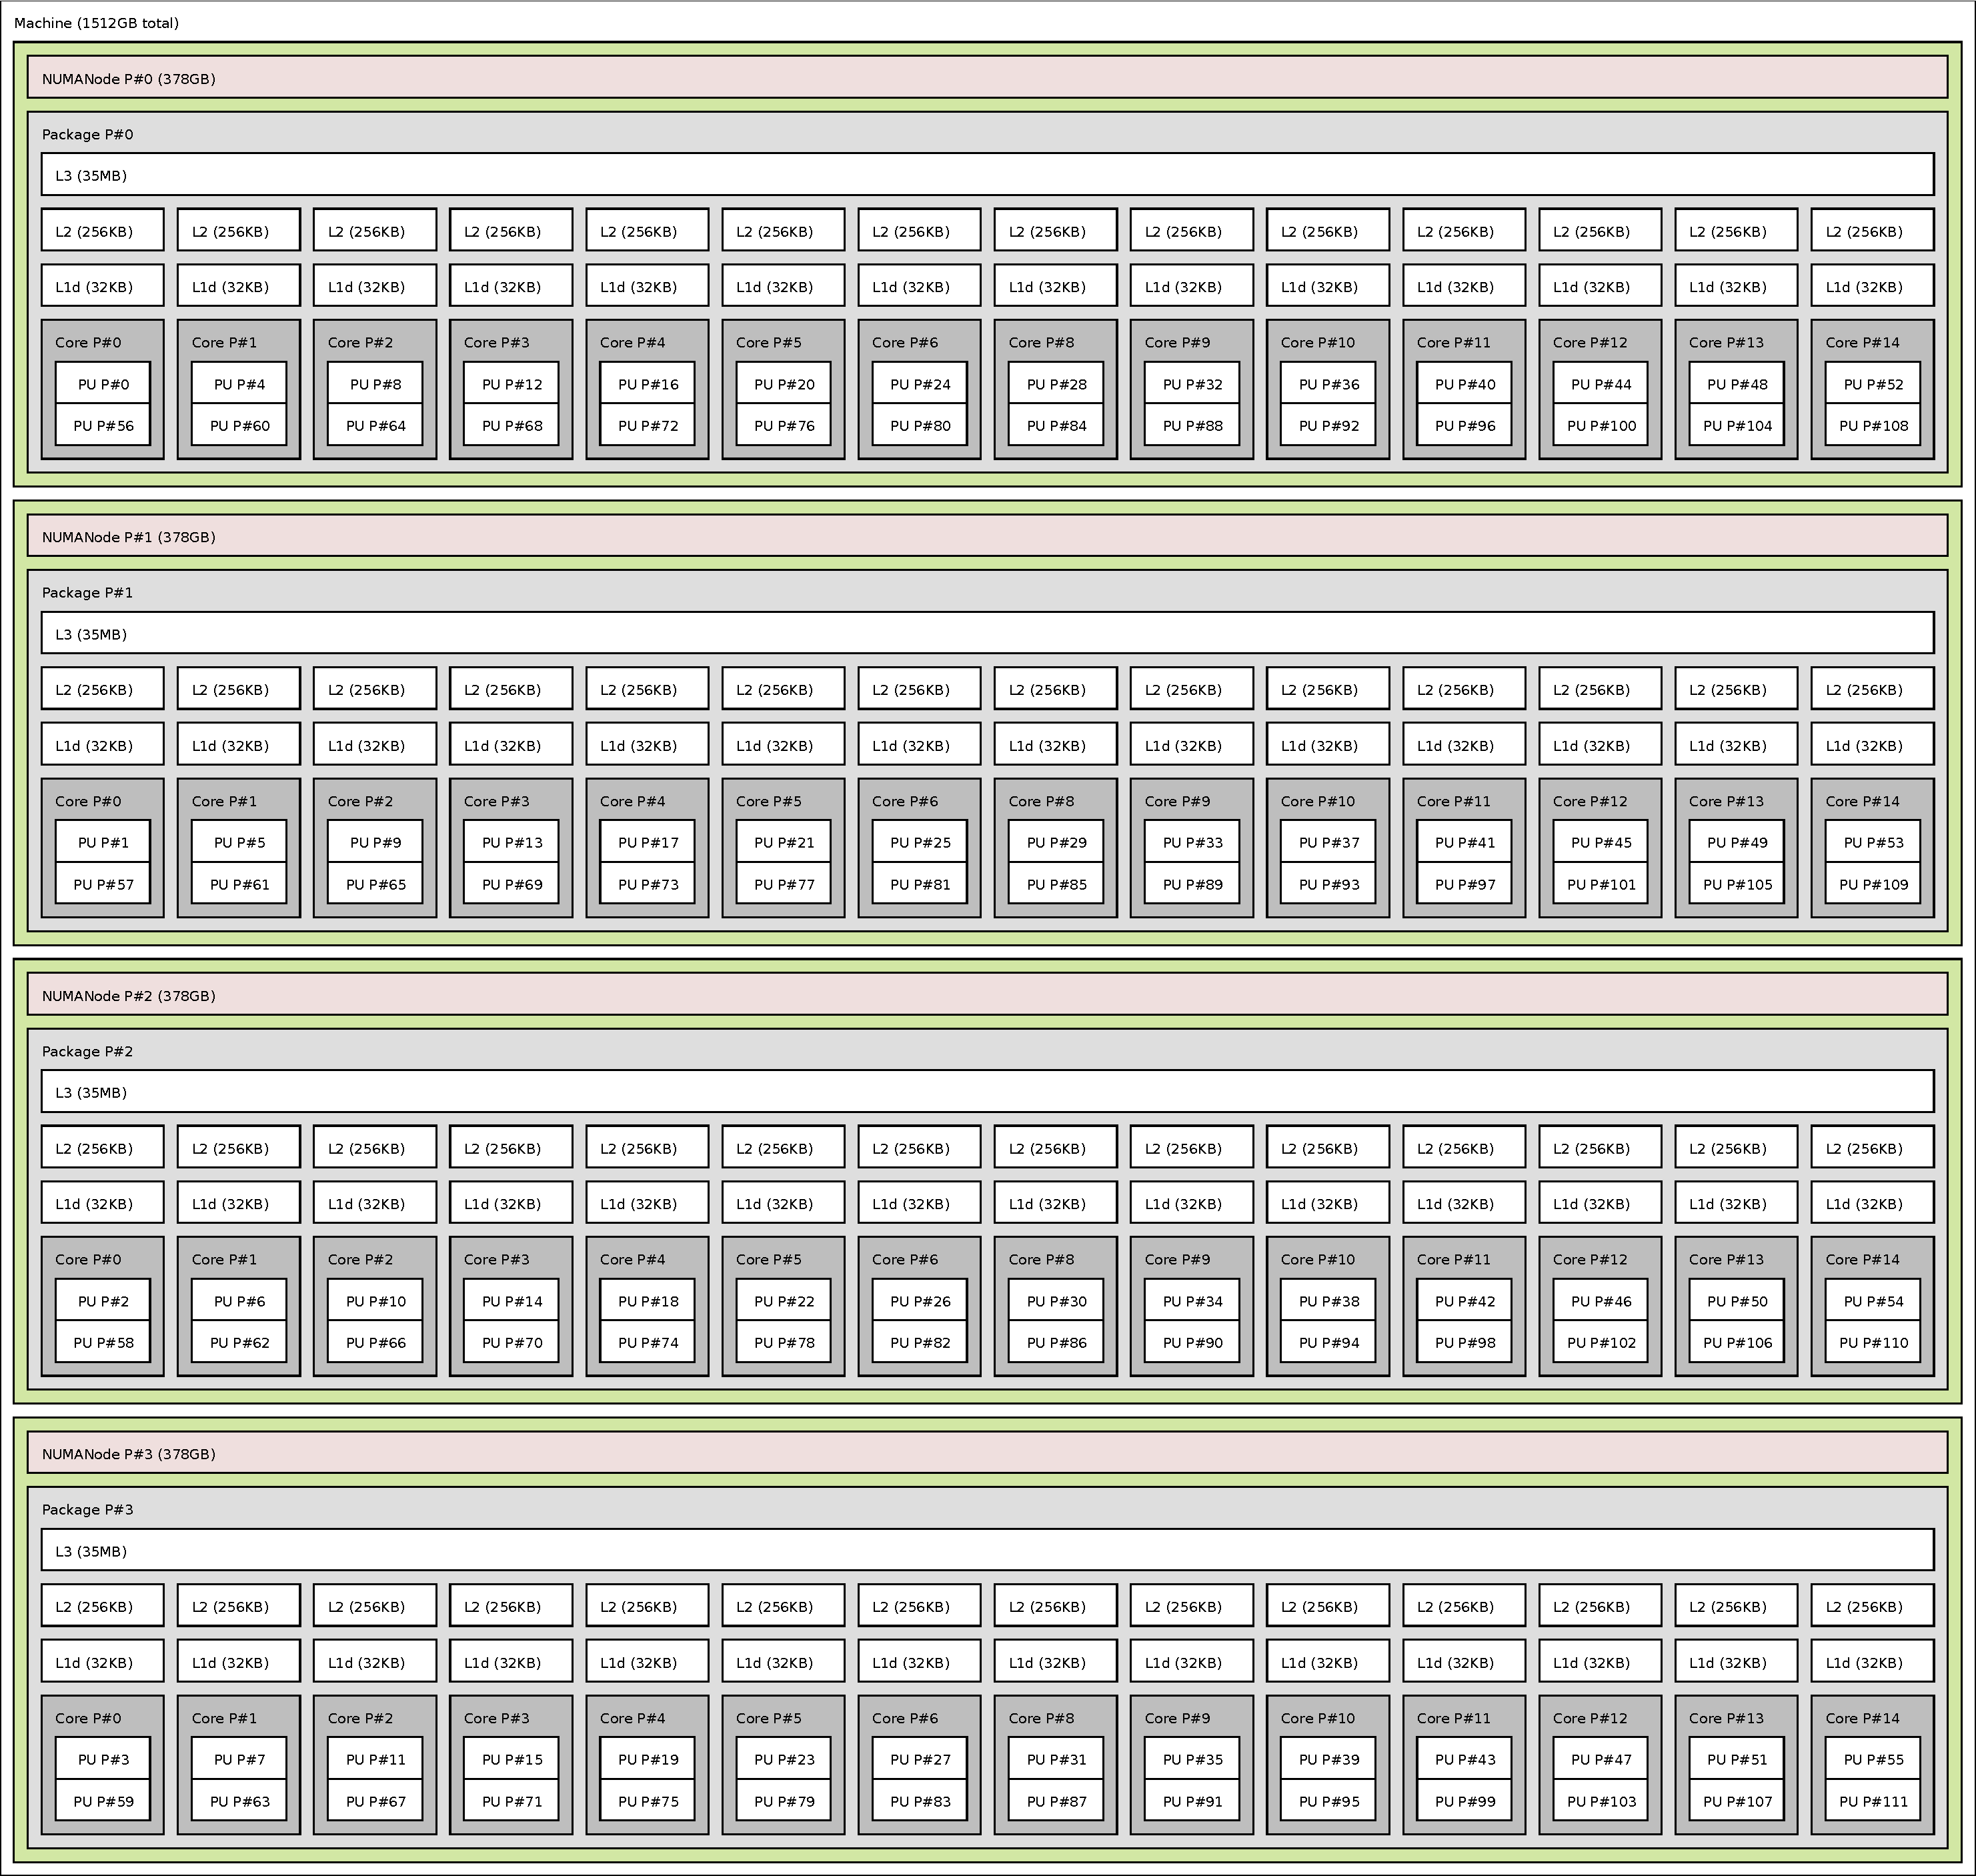
\includegraphics[height=7cm]{lstopo_wurst.pdf}
\end{frame}

\begin{frame}[label=caches]
  \frametitle{Caches: it Takes Up a Lot of Space!}
  \framesubtitle{PowerPC A2}
  \centering
  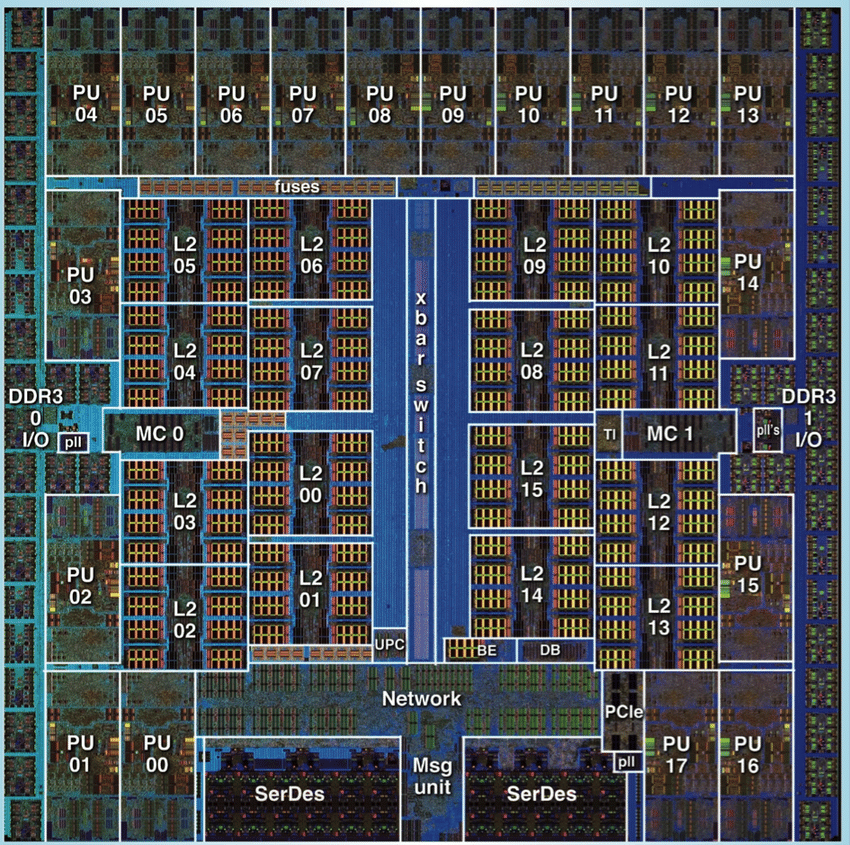
\includegraphics[height=7cm]{die-bgq.png}
\end{frame}


\subsection{Organisation}

% lignes, LRU, 

% cohérence, false sharing

\begin{frame}[label=cache_organization]
\frametitle{Cache Organization}
\framesubtitle{Typical L1 Cache}

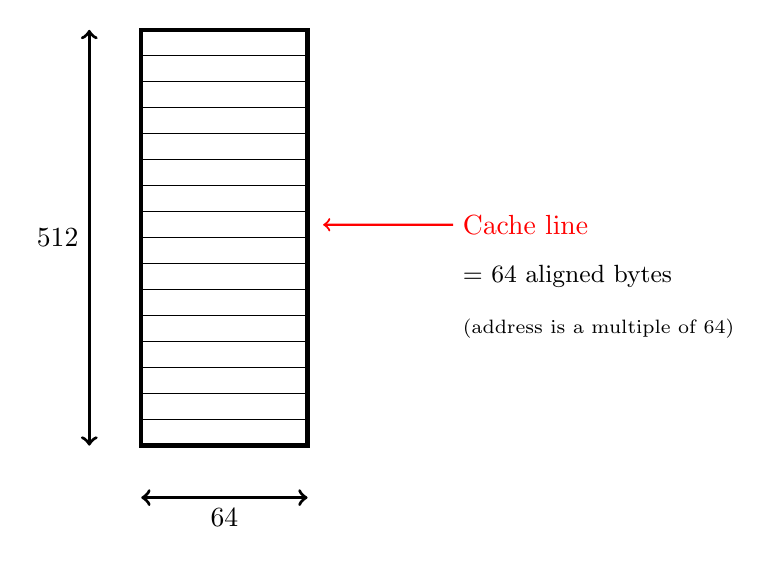
\begin{tikzpicture}[xscale=0.66, yscale=0.33]
  \draw[ultra thick] (0, 0) rectangle +(3.2, 16);
  \foreach \i in {1,2, ..., 15} \draw(0, \i) -- +(3.2, 0);

  \draw[very thick,<->] (-1, 0) -- node[left] {512} +(0, 16);
  \draw[very thick,<->] (0, -2) -- node[below] {64} +(3.2, 0);

  \node[anchor=west, red] at (6, 8.5) (tag) {Cache line};
  \draw[->, red,thick] (tag) -- (3.5, 8.5);

  \node[anchor=west,font=\small] at (6, 6.5) {$=$ 64 aligned bytes};
  \node[anchor=west,font=\scriptsize] at (6, 4.5) {(address is a multiple of 64)};
\end{tikzpicture}
\end{frame}

%%%%%%%%%%%% 

\begin{frame}[label=cache_organization,fragile]
\frametitle{Cache Misses}

 \begin{tikzpicture}[xscale=0.66,yscale=0.33]

   \fill[fill=lightgray] (-9, 19) rectangle +(16, 1);
   \draw (-6.4, 19) -- +(0, 1);
   \draw (-3.2, 19) -- +(0, 1);
   \draw[fill=orange] (-2.4, 19) rectangle +(0.4, 1);
   \draw (0, 19) -- +(0, 1);
   \draw (3.2, 19) -- +(0, 1);
   \draw[fill=green] (4.8, 19) rectangle +(0.4, 1);
   \draw (6.4, 19) -- +(0, 1);

   \draw[ultra thick] (-9, 20) -- +(16, 0);
   \draw[ultra thick] (-9, 19) -- +(16, 0);
   \node[font=\small] at (-1, 21) {RAM};   
   
   \node at (-7, 8) (cpu) {
\includegraphics[width=1cm]{cpu_clipart.png}};
   \node<2-3>[above=0.2cm of cpu] {\mintinline{C}{x = A[i];}};
   \node<4-8>[above=0.2cm of cpu] {\mintinline{C}{y = A[j];}};
   
   \draw<2>[red, thick, ->] (cpu) -- node[above,font=\small] {0x7f6fe2715518} (-0.33, 8);
   \draw[fill=green] (1.6, 0) rectangle +(0.4, 1);

   \draw<4-7>[red, thick, ->] (cpu) -- node[above,font=\small] {0x7fc1353384e0} (-0.33, 8);
   \draw<8>[red, thick, <-] (cpu) -- node[above,font=\small] {0x7fc1353384e0} (-0.33, 8);
   \node<5>[font=\huge] at (5, 8) {???};
   \draw<6>[thick, ->] (-1.6, 18.5) |- (-0.33, 11.5);
   \draw<7->[fill=orange] (0.8, 11) rectangle +(0.4, 1);
   
   \draw<3>[red, thick, <-] (cpu) -- node[above,font=\small] {0x7f6fe2715518} (-0.33, 8);
   \draw<3>[fill=green] (1.6, 0) rectangle +(0.4, 1);
   \draw<3>[fill=green] (-3.5, 6.5) rectangle +(0.4, 1);
   \draw<8>[fill=orange] (-3.5, 6.5) rectangle +(0.4, 1);

   
   \draw[ultra thick] (0, 0) rectangle +(3.2, 16);
   \foreach \i in {1,2, ..., 15} \draw(0, \i) -- +(3.2, 0);
 \end{tikzpicture}
\end{frame}

%%%%%%%%%

\begin{frame}[label=cache_organization]
\frametitle{Cache Misses (continued)}

\begin{columns}
  \begin{column}{2cm}
    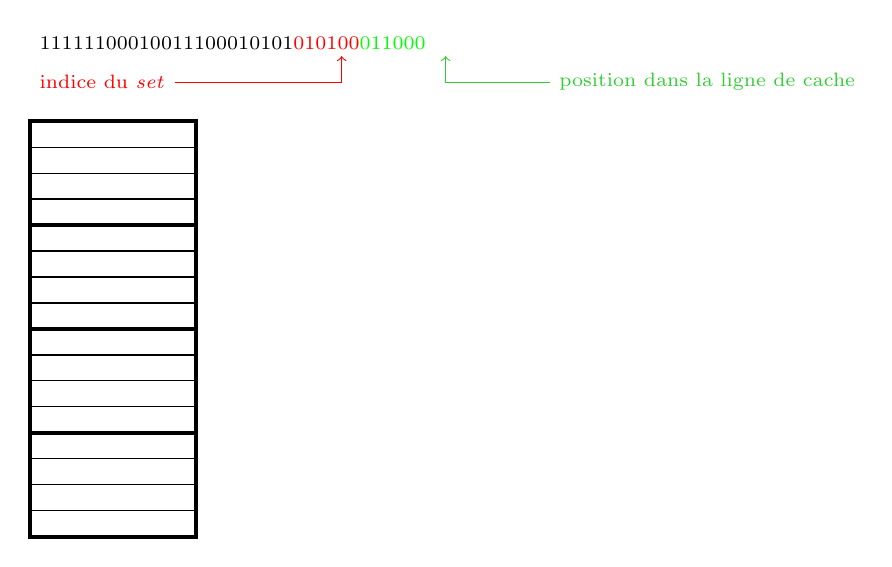
\begin{tikzpicture}[xscale=0.66, yscale=0.33]
      \node[anchor=west,font=\scriptsize] at (0, 19) {11111100010011100010101{\color{red}010100}{\color{green}011000}};

      \node[anchor=west,font=\scriptsize,text=LimeGreen] at (10, 17.5) (pos) {position dans la ligne de cache};

      \node[anchor=west,font=\scriptsize,text=red] at (0, 17.5) (set) {indice du \emph{set}};

      \draw[LimeGreen,->] (pos) -| (8, 18.5);
      \draw[red,->] (set) -| (6, 18.5);
      
      \draw[ultra thick] (0, 0) rectangle +(3.2, 16);
      \foreach \i in {1,2, ..., 15} \draw(0, \i) -- +(3.2, 0);
      \foreach \i in {4,8, 12} \draw<2>[very thick] (0, \i) -- +(3.2, 0);
    \end{tikzpicture}
  \end{column}
  \begin{column}{9cm}
    \begin{block}{In case of cache miss}
    \begin{itemize}
    \item Evict which cache line? 
      \begin{itemize}
      \item LRU, PLRU
      \end{itemize}
    \item What about writes?
      \begin{itemize}
      \item Write-through, write-back
      \item False-sharing
      \end{itemize}
    \item What possible locations for a given line
      \begin{itemize}
      \item Associativity
      \end{itemize}
    \end{itemize}
  \end{block}
\end{column}
\end{columns}
\end{frame}

%%%%%%%%%%%%%%%%

\subsection{Petits exemples}

\begin{frame}[label=applications,fragile=singleslide]
\frametitle{Small Examples}
\framesubtitle{2D array copy}

\begin{minted}[fontsize=\small]{C}
/* Bad */
for (int i = 0; i < N; i++)
    for (int j = 0; j <N; j++)
        dst[j][i] = src[j][i];
\end{minted}

\bigskip

\begin{minted}[fontsize=\small]{C}
/* Good */
for (int i = 0; i < N; i++)
    for (int j = 0; j < N; j++)
        dst[i][j] = src[i][j];
\end{minted}
\end{frame}

%%%%%%%%%%%%%%


\begin{frame}[label=applications,fragile]
\frametitle{Small Examples}
\framesubtitle{Naive GEMM (Matrix-Matrix Product)}

\hrule%
\begin{overlayarea}{\textwidth}{2.5cm}%
\begin{onlyenv}<1>%
\begin{minted}[fontsize=\small]{C}
for (int i = 0; i < N; i++)
  for (int j = 0; j < N; j++)
    for (int k = 0; k < N; k++)
      C[i * N + j] += A[i * N + k] * B[k * N + j];
\end{minted}
\end{onlyenv}%
\begin{onlyenv}<2-3>%
\vspace{-0.45cm}
\begin{minted}[fontsize=\small]{C}
for (int i = 0; i < N; i++)
  for (int k = 0; k < N; k++)
    for (int j = 0; j < N; j++)
      C[i * N + j] += A[i * N + k] * B[k * N + j];
\end{minted}
  \vfill
\end{onlyenv}%
\begin{onlyenv}<4-5>%
  \vspace{-0.45cm}
\begin{minted}[fontsize=\small]{C}
transpose(B);
for (int i = 0; i < N; i++)
  for (int j = 0; j < N; j++)
    for (int k = 0; k < N; k++)
      C[i * N + j] += A[i * N + k] * B[j * N + k];
\end{minted}
\end{onlyenv}%

\end{overlayarea}

\hrule

\begin{overlayarea}{\textwidth}{4cm}

  \begin{onlyenv}<1,3>
  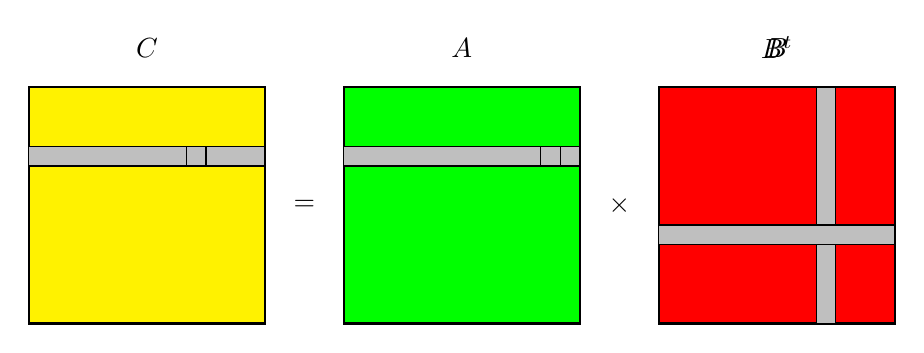
\begin{tikzpicture}
  \node at (1.5, 3.5) {$C$};
  \draw[thick,fill=yellow] (0, 0) rectangle + (3, 3);
  \node at (3.5, 1.5) {$=$};
  \node at (5.5, 3.5) {$A$};
  \draw[thick,fill=green]    (4, 0) rectangle + (3, 3);
  \node at (7.5, 1.5) {$\times$};
  \node<1,3> at (9.5, 3.5) {$B$};
  \node<5> at (9.5, 3.5) {$B^t$};
  \draw[thick,fill=red] (8, 0) rectangle + (3, 3);

  \draw<1,5>[fill=lightgray] (2, 2) rectangle +(0.25, 0.25);
  \draw<3>[fill=lightgray] (0, 2) rectangle +(3, 0.25);
  
  \draw<1>[fill=lightgray] (2, 2) rectangle +(0.25, 0.25);
  \draw<1,5>[fill=lightgray] (4, 2) rectangle +(3, 0.25);
  \draw<3>[fill=lightgray] (6.5, 2) rectangle +(0.25, 0.25);
  \draw<1>[fill=lightgray] (10, 0) rectangle +(0.25, 3);
  \draw<3,5>[fill=lightgray] (8, 1) rectangle +(3, 0.25);
\end{tikzpicture}
\end{onlyenv}

\begin{block}<only@2>{Trick \#1}
\begin{itemize}
\item Swap the loops over $j$ abd $k$
\item[$\Rightarrow$] Contiguous accesses (spatial locality)
\item Bonus: opens vectorization possibilities
\end{itemize}
\end{block}


\begin{block}<only@4>{Trick \#2}
\begin{itemize}
\item Pre-transpose $B$.
  
\item Bonus: opens vectorization possibilities
\end{itemize}
\end{block}

\begin{exampleblock}<only@5>{Bilan}
  \begin{itemize}    
  \item Small matrices: not profitable
    \begin{itemize}
    \item Overhead too high
    \end{itemize}

  \item Large matrices: clear gain
    \begin{itemize}
    \item $N=3200 : 177s \leadsto 63s$.
    \end{itemize}
  \end{itemize}
\end{exampleblock}

\begin{block}<only@6>{Astuce \#3}
  \begin{itemize}
  \item Product by blocks
  
  \item Con: naturally recursive instead of iterative

  \item Pro: small blocks fit in cache
  \item (3 matrices $32 \times 32$ fit)
  \end{itemize}
\end{block}
\end{overlayarea}
\end{frame}


\subsection{Bucket Sort}

%%%%%%%%%%%%%%%%%%%%%%%%%%%%%%%%%%
      \pgfmathdeclarerandomlist{MyRandomColors}{{pink}{red}{orange}{yellow}{green}{cyan}{blue}{magenta}{violet}{lightgray}{darkgray}}

      
\begin{frame}[fragile,label=radix]
  \frametitle{Example: Bucket Sort}

%int C[256];
%for (int i = 0; i < 256; i++)
%    C[i] = 0;

    \begin{columns}[c]
    \begin{column}{.4\textwidth}

\begin{minted}{C}
// Initialization
for (int i = 0; i < M; i++) {
    C[i] = 0;
}

// Histogram
for (int i = 0; i < N; i++) {
    int bucket = f(A[i]);
    C[bucket]++;
}

// Prefix-sum
int s = 0;
for (int i = 0; i < M; i++) {
    P[i] = s;
    s += C[i];
}

// Dispatch
for (int i = 0; i < N; i++) {
    int bucket = f(A[i]);
    B[P[bucket]] = A[i];
    P[bucket]++;
}
\end{minted}
    \end{column}
    \begin{column}{.6\textwidth}


      \begin{tikzpicture}[scale=0.25, >={To[sep]}]
        \path[red,dotted,use as bounding box] (-1, 0) rectangle +(26, 32);
        
        % état initial aléatoire
        \pgfmathsetseed{57}
        \foreach \i in {0, 1, ..., 31} {
          \pgfmathrandomitem{\RandomColor}{MyRandomColors} 
          \fill[fill=\RandomColor] (0, \i) rectangle +(3, 1);
        }
        \draw[thick] (0, 0) rectangle +(9, 32);
        \draw[thick] (3, 0) -- +(0, 32);
        \foreach \i in {1, ..., 31} {
          \draw (0, \i) -- +(9, 0);
        }
        \foreach \i / \l in {0/3, 1/0, 2/7, 3/1, 4/10, 5/2, 6/5, 7/2, 8/10, 9/5,
          10/2, 11/3, 12/8, 13/7, 14/9, 15/10, 16/3, 17/6, 18/4, 19/6,
          20/10, 21/0, 22/5, 23/3, 24/5, 25/9, 26/5, 27/7, 28/8, 29/9,
          30/8, 31/5} {
%          \node[font=\tiny] at (-1, 31.5-\i) {\i};
          \node[font=\tiny] at (4, 31.5-\i) {\l};
        }
        
        % côté droit : trié
        \begin{scope}[xshift=16cm]
          % situation finale supposée
          \begin{onlyenv}<1-3>
          \fill[fill=pink] (0, 30) rectangle +(3, 2);
          \fill[fill=magenta] (0, 29) rectangle +(3, 1);
          \fill[fill=violet] (0, 26) rectangle +(3, 3);
          \fill[fill=blue] (0, 22) rectangle +(3, 4);
          \fill[fill=cyan] (0, 21) rectangle +(3, 1);
          \fill[fill=green] (0, 15) rectangle +(3, 6);
          \fill[fill=yellow] (0, 13) rectangle +(3, 2);
          \fill[fill=orange] (0, 10) rectangle +(3, 3);
          \fill[fill=red] (0, 7) rectangle +(3, 3);
          \fill[fill=lightgray] (0, 4) rectangle +(3, 3);
          \fill[fill=darkgray] (0, 0) rectangle +(3, 4);
        \end{onlyenv}

        % \begin{onlyenv}<4->
        %     \fill[very nearly transparent, fill=pink] (0, 30) rectangle +(3, 2);
        %     \fill[very nearly transparent, fill=magenta] (0, 29) rectangle +(3, 1);
        %     \fill[very nearly transparent, fill=violet] (0, 26) rectangle +(3, 3);
        %     \fill[very nearly transparent, fill=blue] (0, 22) rectangle +(3, 4);
        %     \fill[very nearly transparent, fill=cyan] (0, 21) rectangle +(3, 1);
        %     \fill[very nearly transparent, fill=green] (0, 15) rectangle +(3, 6);
        %     \fill[very nearly transparent, fill=yellow] (0, 13) rectangle +(3, 2);
        %     \fill[very nearly transparent, fill=orange] (0, 10) rectangle +(3, 3);
        %     \fill[very nearly transparent, fill=red] (0, 7) rectangle +(3, 3);
        %     \fill[very nearly transparent, fill=lightgray] (0, 4) rectangle +(3, 3);
        %     \fill[very nearly transparent, fill=darkgray] (0, 0) rectangle +(3, 4);
        %   \end{onlyenv}

          % items qui arrivent en cours de route
          \fill<5->[fill=blue] (0, 25) rectangle +(3, 1);
          \fill<9->[fill=pink] (0, 31) rectangle +(3, 1);
          \fill<11->[fill=orange] (0, 12) rectangle +(3, 1);
          
          % cadre
          \draw[thick] (0, 0) rectangle +(9, 32);
          \draw[thick] (3, 0) -- +(0, 32);
          \foreach \i in {1, ..., 31} {
            \draw (0, \i) -- +(9, 0);
          }
      \end{scope}

      % taille des buckets
      \begin{onlyenv}<2>
        \draw[<->] (15, 30) -- node[left] {$C[0]$} +(0, 2);
        \draw[<->] (15, 26) -- node[left] {$C[2]$} +(0, 3);
        \draw[<->] (15, 22) -- node[left] {$C[3]$} +(0, 4);
        \draw[<->] (15, 15) -- node[left] {$C[5]$} +(0, 6);
        \draw[<->] (15, 13) -- node[left] {$C[6]$} +(0, 2);
        \draw[<->] (15, 10) -- node[left] {$C[7]$} +(0, 3);
        \draw[<->] (15, 7) -- node[left] {$C[8]$} +(0, 3);
        \draw[<->] (15, 4) -- node[left] {$C[9]$} +(0, 3);
        \draw[<->] (15, 0) -- node[left] {$C[10]$} +(0, 4);
      \end{onlyenv}

      % pointeurs initiaux sur les buckets
      \begin{onlyenv}<3->
        \draw<-8>[->] (15, 31.5) node[left] {$P[0]$} -- (16, 31.5);
        \draw[->] (15, 28.5) node[left] {$P[2]$} -- (16, 28.5);
        \draw<-5>[->] (15, 25.5) node[left] {$P[3]$} -- +(1, 0);
        \draw[->] (15, 20.5) node[left] {$P[5]$} -- (16, 20.5);
        \draw[->] (15, 14.5) node[left] {$P[6]$} -- (16, 14.5);
        \draw<-11>[->] (15, 12.5) node[left] {$P[7]$} -- (16, 12.5);
        \draw[->] (15, 9.5)  node[left] {$P[8]$} -- (16,  9.5);
        \draw[->] (15, 6.5)  node[left] {$P[9]$} -- (16,  6.5);
        \draw[->] (15, 3.5)  node[left] {$P[10]$}-- (16,  3.5);
      \end{onlyenv}
    
      % pointeurs modifiés
      \draw<6->[->] (15, 24.5) node[left] {$P[3]$} -- +(1, 0);
      \draw<9->[->] (15, 30.5) node[left] {$P[0]$} -- +(1, 0);
      \draw<12->[->] (15, 11.5) node[left] {$P[7]$} -- +(1, 0);
      
      % flèches de progression à gauche
      \draw<4-5>[thick,->] (-2, 31.5) -- +(2, 0);
      \draw<7-8>[thick,->] (-2, 30.5) -- +(2, 0);
      \draw<10-11>[thick,->] (-2, 29.5) -- +(2, 0);

      \draw<5>[->] (9, 31.5) -- (10, 30.5) -- (10, 27) -- (14, 27) -- (16, 26);
      \draw<8>[->] (9, 30.5) -- (14, 30.5) -- (16, 31);
      \draw<11>[->] (9, 29.5) -- (10, 29.5) -- (10, 13.5) -- (14, 13.5) -- (16, 13);
      
\end{tikzpicture}
  
      
    \end{column}
  \end{columns}
\end{frame}

%%%%%%%%%%%%%%%%%%%%%%%%%%%%%%%%%%

\begin{frame}[fragile=singleslide]
  \frametitle{Bucket Sort: Analyse}


  \begin{exampleblock}{Histogram phase}
    \begin{itemize}
    \item Does $C$ fit in cache? 
    \item \# buckets $\times$ \mintinline[fontsize=\normalsize]{C}{sizeof(int)} $\leq$ 32KB ?
    \item \# buckets $\leq$ 8192 \raisebox{-2pt}{
\includegraphics[height=\baselineskip]{Content.png}}
    \end{itemize}
  \end{exampleblock}

  \medskip

  \begin{alertblock}{Dispatching Phase}
    \begin{itemize}
    \item Write into \#buckets (\alert{far apart}) addresses 
    \item One bucket $\leftrightarrow$ one cache line
    \item \# buckets $\leq$ 512 \raisebox{-2pt}{
\includegraphics[height=\baselineskip]{Content.png}}
    \item \scriptsize Requires $C$ + target in cache
    \end{itemize}
  \end{alertblock}  
\end{frame}

%%%%%%%%%%%%%%%%%%%%%%%%%%%%%%%%%%%%%%%%%%%%%%%%%%%%%%%%%%%%%%

\begin{frame}[fragile=singleslide]
  \frametitle{GEMV (matrix-vector product)}

  \begin{block}{Direct version}
\begin{minted}{C}
/* y += A*x */
void gemv(int n, int m, double * A, int ldA, double * x, double * y)
{
    for (int i = 0; i < m; i++)
        for (int j = 0; j < n; j++)
            y[i] += A[i * ldA + j] * x[j];
}
\end{minted}
    \begin{itemize}
    \item Reads $A$ at 7GB/s on my laptop
    \item 50\% of peak memory bandwidth
    \end{itemize}
  \end{block}
\end{frame}

%%%%%%%%%%%%%%%%%%%%%%%%%%%%%%%%%%%%%%%%%%%%%%%%%%%%%%%%%%%%%%%%%%%%

\begin{frame}[fragile=singleslide]
  \frametitle{GEMV (matrix-vector product)}

\begin{alertblock}{Blocked version}
\begin{minted}{C}
static const int nb = 8;
void gemvb(int n, int m, int double *A, int ldA, double *x, double * y)
{
    int nhi = (n / nb) * nb;
    int mhi = (m / nb) * nb;
    int nextra = n - nhi;
    int mextra = m - mhi;
    for (int i = 0; i < mhi; i += nb) {
        for (int j = 0; j < nhi; j += nb)
            gemv(nb, nb, stride, &A[i*ldA + j], &x[j], &y[i]);
        gemv(nb, nextra, stride, &A[i*ldA + nhi], &x[nhi], &y[i]);
    }
    for (int j = 0; j < nhi; j += nb)
        gemv(nb, mextra, stride, &A[mhi*ldA + j], &x[j], &y[mhi]);
    gemv(mextra, nextra, stride, &A[mhi*ldA + nhi], &x[nhi], &y[mhi]);
}
\end{minted}
    \begin{itemize}
    \item Reads $A$ at 15GB/s on my laptop
    \item 100\% of peak memory bandwidth
    \item $2\times$ faster than naive algorithm
    \end{itemize}

\end{alertblock}
\end{frame}

%%%%%%%%%%%%%%%%%%%%%%%%%%%%%%%%%%%%%%%%%%%%%%%%%%%%%%%%%%%%%%

\begin{frame}[fragile]
  \frametitle{SpMV (sparse GEMV): the cursed operation}

\begin{minted}{C}
for (long k = 0; k < nnz; k++) {
    int i = transpose ? Mj[k] : Mi[k];
    int j = transpose ? Mi[k] : Mj[k];
    double v = Mx[k];
    double a = y[i];              // risk
    double b = x[j];              // risk
    y[i] = a + b * v;
}
\end{minted}

  \begin{itemize}
  \item Sort \texttt{Mi} $\leadsto$ misses on $x$
  \item Sort \texttt{Mj} $\leadsto$ misses on $y$    
  \item Using \textbf{blocks} of vectors \red{amortize} misses
  \item `` Reasonable'' idea: use blocks of the size of a cache line
  \end{itemize}
\end{frame}

%%%%%%%%%%%%%%%%%%%%%%%%%%%%%%%%%%%%%%%%%

\begin{frame}
  \frametitle{Can We Observe All These Phenomena?}

  \begin{exampleblock}{Yes!}
    \begin{itemize}
    \item Execution: `` events'' (cache miss, etc.)
    \item These events have \textbf{names}...
      \begin{itemize}
      \item ... that vary from one system / mechanism to another
      \end{itemize}
    \item Hardware counter $\leadsto$ mesure
    \item Not very easy to access and not very portable (OS / CPU-specific)
    \end{itemize}
  \end{exampleblock}
  
  \begin{block}{Under Linux, with \texttt{perf}}
    \begin{itemize}
    \item Available event list: \texttt{perf list}
      \begin{itemize}
      \item \texttt{cpu-cycles}, \texttt{instructions}, \texttt{L1-dcache-load-misses}, ...
      \end{itemize}
    \item \texttt{perf stat -e [list evt] ./prog}
    \item \texttt{perf record -e [list evt] ./prog} then \texttt{perf report}
    \end{itemize}
  \end{block}

  + profiling with \texttt{score-p}
\end{frame}

%%%%%%%%%%%%%%%%%%%%%%%%%%%%%%%%%%%%%%%%%%%%%%%%%%

\begin{frame}
  \frametitle{Can We Observe All These Phenomena?}


  \begin{alertblock}{Manual Instrumentation with the \texttt{PAPI} library}
    \begin{itemize}
    \item Performance API (Application Programming Interface)
    \item Documentation USED TO BE unreadable
    \item New version 7.0
    \item New high-level API
    \item Command-line tool \texttt{papi\_avail} list events
      \begin{itemize}
      \item \texttt{PAPI\_L1\_DCM  : Level 1 data cache misses}
      \end{itemize}
    \item Then instrument your code...
    \item \textbf{Do} read ``\textit{Redesigning PAPI’s High-Level API}'', Frank Winkler
    \end{itemize}
  \end{alertblock}
\end{frame}


  %%%%%%%%%%%%%%%%%%%%%%%%%%%%%%% 

\begin{frame}[fragile=singleslide]
  \frametitle{PAPI in Action}
  
\begin{minted}{C}
#include <err.h>
#include <papi.h>
  
int main()
{
  int retval;
  retval = PAPI_hl_region_begin("computation");
  if (retval != PAPI_OK)
       errx(1, "something went wrong");

  // HERE: observed code 

  retval = PAPI_hl_region_end ("computation");
  if (retval != PAPI_OK)
      ....
\end{minted}

\begin{itemize}
\item Control using environment variables (\texttt{PAPI\_EVENTS})
\item Write result in a file
\item Can also use to low-level API to get results inside the code
\end{itemize}


\end{frame}
  
\end{document}


%%% Local Variables:
%%% TeX-command-extra-options: "-shell-escape"
%%% TeX-engine: xetex
%%% ispell-local-dictionary: "english"
%%% eval: (flyspell-mode 1)
%%% eval: (reftex-mode 1)
%%% End:
